% \documentclass[12pt, openright]{report}
\documentclass[12pt, headinclude, parskip=half+, numbers=noenddot, openright]{scrreprt}
% PDF-Kompression
\pdfminorversion=5
\pdfobjcompresslevel=1
% Allgemeines
\usepackage[automark]{scrpage2} % Kopf- und Fußzeilen
% \usepackage{amsmath,marvosym} % Mathesachen
\usepackage[T1]{fontenc} % Ligaturen, richtige Umlaute im PDF
\usepackage[utf8]{inputenc}% UTF8-Kodierung für Umlaute usw
% Schriften
\usepackage{setspace} % Zeilenabstand
\usepackage{titlesec}
\onehalfspacing % 1,5 Zeilen
% Schriften-Größen
\setkomafont{chapter}{\Large\rmfamily} % Überschrift der Ebene
\setkomafont{section}{\large\rmfamily}
\setkomafont{subsection}{\large\rmfamily}
\setkomafont{subsubsection}{\normalsize\rmfamily}
\setkomafont{chapterentry}{\large\rmfamily} % Überschrift der Ebene in Inhaltsverzeichnis
\setkomafont{descriptionlabel}{\bfseries\rmfamily} % für description Umgebungen
\setkomafont{captionlabel}{\small\bfseries}
\setkomafont{caption}{\small}
% Language: English
\usepackage[english]{babel}
% PDF
\usepackage[final]{microtype} % mikrotypographische Optimierungen
\usepackage{float}
\usepackage{url} % ermögliche Links (URLs)
\usepackage{pdflscape} % einzelne Seiten drehen können
\usepackage{hyperref}
% Tabellen
\usepackage{multirow} % Tabellen-Zellen über mehrere Zeilen
\usepackage{multicol} % mehre Spalten auf eine Seite
\usepackage{tabularx} % Für Tabellen mit vorgegeben Größen
\usepackage{longtable} % Tabellen über mehrere Seiten
\usepackage{array}
%  Bibliographie
% Sort by order of appearance in document
\usepackage[sorting=none]{biblatex}
% Bilder
\usepackage{graphicx} % Bilder
\usepackage{color} % Farben
\usepackage{wrapfig}
\usepackage[all]{hypcap} % Beim Klicken auf Links zum Bild und nicht zu Caption gehen
% Bildunterschrift
\setcapindent{0em} % kein Einrücken der Caption von Figures und Tabellen
\setcapwidth{0.9\textwidth} % Breite der Caption nur 90% der Textbreite, damit sie sich vom restlichen Text abhebt
\setlength{\parskip}{0pt}
\setlength{\abovecaptionskip}{0.2cm} % Abstand der zwischen Bild- und Bildunterschrift
% Quellcode
% für Formatierung in Quelltexten, hier im Anhang
\usepackage{listings}
\definecolor{grau}{gray}{0.25}
\lstset{
	extendedchars=true,
	basicstyle=\normalsize\ttfamily,
	tabsize=2,
	keywordstyle=\textbf,
	commentstyle=\color{grau},
	stringstyle=\textit,
	numbers=left,
	numberstyle=\tiny,
	% für schönen Zeilenumbruch
	breakautoindent  = true,
	breakindent      = 2em,
	breaklines       = true,
	postbreak        = ,
	prebreak         = \raisebox{-.8ex}[0ex][0ex]{\Righttorque},
}
% linksbündige Fußboten
\deffootnote{1.5em}{1em}{\makebox[1.5em][l]{\thefootnotemark}}
% prevent footnotes from being split over multiple pages
\interfootnotelinepenalty=10000

\typearea{14} % typearea berechnet einen sinnvollen Satzspiegel (das heißt die Seitenränder) siehe auch http://www.ctan.org/pkg/typearea. Diese Berechnung befindet sich am Schluss, damit die Einstellungen oben berücksichtigt werden

\usepackage{scrhack} % Vermeidung einer Warnung



\addbibresource{references.bib}



\begin{document}



\pagenumbering{Roman}
\pagestyle{empty} % remove header and footer for first page

% title page
\clearscrheadings\clearscrplain
\begin{center}

HTW Berlin\\
University of Applied Sciences

\vspace{2cm}

Bachelor's Thesis

\vspace{1cm}

\begin{Large}
  Chatbots: Development and Applications
  \vspace{3cm}
\end{Large}

\begin{tabular}{rl}
{\bfseries Author} & Jorin Vogel\\
{\bfseries First Examiner} & Prof. Dr. Gefei Zhang\\
{\bfseries Second Examiner} & Prof. Dr. Carsten Busch\\
\end{tabular}

\vspace{3cm}

International Media and Computing\\
Faculty IV

\vspace{6cm}

July 29, 2017

\end{center}

\clearpage

% TODO: think about adding an abstract and a licensing notice


\tableofcontents
% \listoffigures
% \listoftables

% \chapter{Introduction}


TODO

% Notes:

% -	What's the problem to be solved?
% -	Why is it a problem?
% -	How do I intent to solve it?
% -	How will this help the world?
% -	How is this work structured?


% There have been many headlines about chatbots in recent time; yet still few people use them in their daily lives. That makes it uncertain in which businesses chatbots and their conversational user interfaces may be an improvement over the current, graphical interfaces.

% In this thesis I would like to develop a chatbot specifically with the goal in mind to create a product people would actually use. Additionally, building on the experience of implementing a practical chatbot, I would like to research what applications chatbots are most suitable for and under which circumstances a chatbot is less beneficial.

% -	What are chatbots?
% -	What have people done with them?
% -	What can they be used for?
% -	Why would you use them?
% -	Why are they so hyped?
% -	How do you use them?
% -	Which platform is best for me?
% -	How to develop one?
% -	What are they really good at?
% -	What are they not good at?
% -	What can we expect from the future?

\pagestyle{useheadings} % enable header and footer for other pages
\pagenumbering{arabic}
\chapter{Fundamentals}


Before working on a topic it is necessary to have common definitions of its vocabulary. This chapter helps aligning previous assumptions.

\section{Definition Chatbot}
\label{defchatbot}


The term \emph{chatbot} consists of two other terms - \emph{chat} and \emph{bot}.
The meaning can be better understood by examining the two components separately.
\\

The Oxford Dictionary defines \textbf{chat} as ``an informal conversation'' and more specifically as ``the online exchange of messages in real time with one or more simultaneous users of a computer network''~\cite{oxfordchat}.
\\
As apparent in this definition, conversations play a central role in \emph{chat} and therefore \emph{chatbots}.
Other noteworthy aspects of this definition are the inherent \emph{informal} format of a \emph{chat},
and the traits of being \emph{online} and \emph{real time}.
\\

Informality doesn't have to be seen as a strict requirement; however a chat message and, for example, a classical letter have different degrees of formality.
\\

Being \emph{online} and thereby not bound to a specific geographic location, device or other physicality can be seen as critical foundation for determining potential types of systems suitable for such media.
\\

The aspect of limiting communication to \emph{real time} implies restrictions on possible interactions and sets a baseline for the expected user experience.
This also excludes the usage of certain technologies that don't allow for the desired responsiveness.
\\

A \emph{conversation} is defined as ``a talk, especially an informal one, between two or more people, in which news and ideas are exchanged''~\cite{oxfordconversation}.
\\
Fundamental to this definition is that there are always at least \emph{two} parties involved in communication and that information is \emph{exchanged}.
Keeping that in mind, the kind of systems involved in this should always receive and provide information;
chatbots can not work with solely unidirectional interaction.
\\

\textbf{Bot} is defined as being ``(chiefly in science fiction) a robot'' with the specific characteristics of representing ``an autonomous program on a network (especially the Internet) which can interact with systems or users, especially one designed to behave like a player in some video games''~\cite{oxfordbot},
\\

Foremost this provides the information that \emph{bots}, including \emph{chatbots}, are \emph{programs}.
The creation of a chatbot is eventually the creation of an artifact in the form of a computer program.
\\

Furthermore the aspect of \emph{autonomy} and the communication over a \emph{network} can be connected with the previous described trait of a \emph{chat} to be \emph{online}.
\\
The program is given autonomy by not being bound to any specific device.
Building on this allows for different solutions than a scenario where the user is in full control of a program's behavior.
\\

Lastly there is a hint in this definition pointing out that a \emph{bot} can often be seen as a \emph{player} in a \emph{game}.
This trend towards \emph{game-like} mechanisms and the previous mentioned \emph{informality} suggest the utilization of playful interactions.
\\

Concluding from the combination of these definitions, a chatbot can be defined as an autonomous computer program that interacts with users or systems online and in real time in the form of, often play-like and informal, conversations.

\section{Conversational Interfaces}


Having defined the concept and character of chatbots, one apparent attribute of the technology under examination is that its domain of application involves interaction with one or more users.
\\

Any form of interaction requires an \emph{interface} as a way to interact.
An \textbf{interface} is generally described as a ``point where two systems, subjects, organizations, etc. meet and interact'' and in the area of computing it can be further defined as a ``device or program enabling a user to communicate with a computer''~\cite{oxfordinterface}.
\\

This definition leaves a broad array of possible manifestations.
However, the range of suitable means of communication can be further narrowed by including another aspect of the previous definition, namely that interaction happens in the form of \emph{conversation}.
\\

Many communication mechanisms can be excluded by focusing on this characteristic of the interaction.
\\
The term \emph{conversation} strongly suggests the usage of natural human language as the base for interaction
while discouraging the idea of using an interface consisting purely of static or graphical elements.
\\
Further, conversations are not limited to written language.
Verbal conversation is also a possible interface for communication.
\\

Focusing on written, text-based communication, it becomes apparent that not all text-based interfaces fit the characteristics of a \emph{conversational interface}.
\\
Classical command line interfaces, which are often used to interact with computers, are one example of text-based interfaces that do not have the attributes of conversational interfaces.
As implied in the naming, these interfaces use \emph{commands} for interaction. A \textbf{command} is an ``authoritative order''~\cite{oxfordcommand} which contrasts with a conversation.
\\
The term \emph{conversation} has a connotation of complex, non-linear communication where each involved party understands the underlying ideas communicated opposed to merely receiving the characters the words consist of.
\\

Understanding of the intentions a user has and the ability to adjust interactions accordingly, sets conversational interfaces, and thus chatbots, apart from other text-based interfaces.

\chapter{Applications}


This chapter explores different applications of chatbots
to understand what a chatbot is in practice and to see the kind of applications chatbots can be used for.
\\
Starting with past work and looking at the present in subsequent sections,
different approaches and products are presented.
\\
Furthermore todays ecosystem is portrayed,
which includes an overview about available platforms,
existing products
and current approaches for the creation of chatbots.
\\
Lastly aspired goals, potentials and promises of chatbots are further identified.

\section{Past Work}


Before working on new projects with nowadays technology one should know about prior work and learn from past ideas - both, succeed and failed attempts.
\\
This chapter presents selected events from the last century, which introduced ideas forming the present definition of chatbots.
\\
It should be noted that this is no attempt at presenting an all-encompassing overview about the history of computing, instead the aim is to explain where the idea of chatbots and the interest of creating them originated from.


\subsection{The Turing Test}

Even before the term \emph{chatbot} was coined people started working on machines that interact with humans.
\\
One of the first important milestones was the 1950 paper "Computing Machinery and Intelligence" by Alan Turing\cite{turing}. His ideas back then are still an important building block of what is call a \emph{chatbot} in todays world and his thoughts are still central to many discussions about artificial intelligence.
\\
The most famous idea from this paper is the so called "Turing Test". This test is meant to identify if a machine posses human-like intelligence.
\\
Originally Turing described this test as "imitation game" whereas the experiment consist of a human interacting with two parties via \emph{textual messages}. One of the parties is another human and one is a machine. The human doesn't know upfront which one is the machine, but only that one of them will be a machine. During the \emph{game} the human can interact, via what we nowadays call \emph{chatting}, with the other party and is free to use any variation of messages. If the human is not able to tell which of the two parties is a machine and which one is a human, the machine passes the Turing Test.
\\
When creating a chatbot or another kind of artificial intelligence this test can still be applied to test the human-likeliness of the created machinery. Up to this point in time the Turing Test still remains to be challenged by new systems.


\subsection{ELIZA}

14 Years after the Turing Test was defined Joseph Weizenbaum started working on what would be known as the first program to pass a (limited) version of the Turing Test. Joseph Weizenbaum began working at MIT Artificial Intelligence Laboratory in 1964 and he released the ELIZA program in 1966.
\\

The original version of ELIZA was written in a programming programming language called MAD-Slip which was also created by Joseph Weizenbaum himself and it ran on the IBM 704 computer.
\\
ELIZA creates responses to natural language messages a user inputs via a text-based terminal.
\\

The most famous implementation of ELIZA is called DOCTOR and simulates a Rogerian psychotherapist. Rogerian psychotherapy is a person-centered therapy intended to let the client realize their own attitudes and behavior. Relying on mostly simple methods, it remains a popular treatment. Most answers the therapist gives are questions for further details about information which the client mentioned previously. Furthermore clients mostly keep the assumption that a therapist has specific intentions even when asking a non-obvious question.
\\

ELIZA takes advantage of the structure of the English language; the program takes apart sentences via pattern matching and keywords and reuses phrases after substituting certain words.
\\
For example, a clients answer ``Well, my boyfriend made me come here.'' can be transformed to ``Your boyfriend made you come here?''\cite{elizatest}.
\\
Certain signal words or sentences containing no signals words can be answered with generic, static phrases. Detecting the signal word ``alike'' in the sentence ``Men are all alike.'' ELIZA could pick the programmed phrase ``In what way?'' as answer\cite{elizatest}.
\\

Knowing about the nature of Rogerian psychotherapy, Joseph Weizenbaum created ELIZA initially intended as a parody showing off the simple behavior necessary to imitate this therapy.
\\
He was surprised that even people knowing about the inner workings of the program ended up having serious conversations with ELIZA. In one anecdote Joseph Weizenbaum tells how his secretary, after starting a conversation with ELIZA, asked him: ``Would you mind leaving the room, please?''\cite[5]{weizenbaum}.
\\

Lead by the success of the experiment he published the book "Computer power and human reason: from judgment to calculation" in 1976 which discusses his thoughts about artificial intelligence including the differences between machines and humans and the limits of computer intelligence.
\\
In the book he admits that he had not realized ``that extremely short exposures to a relatively simple computer program could induce powerful delusional thinking in quite normal people.''\cite{bbcnowthen}. This idea coined the term \emph{Eliza Effect} which describes people assuming computers to behave like humans. This term is still in use today.


\subsection{After 1970}

Another famous program was published by the psychiatrist Kenneth Colby in 1972.
\\
He created PARRY as an attempt to simulate a human with paranoid schizophrenia. The implementation of PARRY is far more complex than ELIZA and it also models a personality including concepts of how to have conversations.
\\
The most famous demonstration of PARRY was at the first International Conference on Computer Communications (ICCC) in 1972 where PARRY and ELIZA had a conversation with each other.\cite{internethistory}
\\
Later on in scientific experiments PARRY also passed a version of the Turing Test.
\\

Further programs that have been created to pass the Turing Test and which gained the publics attention include
\\
\emph{Jabberwacky} which was started in 1988 and attempts to learn from the users input\cite{jabberwacky},
\\
\emph{Dr. Sbaitso} which was released in 1991 as an ELIZA-like demonstration for a sound card and was one of the first chatbots for MS-DOS based personal computers\cite{pcmag},
\\
and A.L.I.C.E., which has been first released in 1995 and became famous for its realistic behavior that is based on heuristic patterns instead of static rules\cite{approximatinglife}.
\\

The origin of the term \emph{chatbot} itself can be seen in a paper called ``ChatterBots, TinyMuds, and the Turing Test: Entering the Loebner Prize Competition'' published by Michael L. Mauldin in 1994, whereby \emph{chatbot} can be seen as a variation of the original version \emph{ChatterBots}.\cite{aiconf}
\\

Up until today the Turing Test has only been passed limited to certain domains and there is no chatbot yet that is able to simulate general human behavior indistinguishably from a real human.
\\
It needs to be noted that although creating an as human-like as possible system remains a popular challenge, not all applications of chatbots profit from this type of behavior. Many systems are instead optimized to provide quick and efficient interactions and behave accordingly without attempting to hide their artificiality.

\section{Present Day}
\label{presentday}


With more than sixty years of history the concept of chatbots is not new.
\\
People have been fascinated with the idea of being able to \emph{talk to computers} since a long time;
but past attempts have mostly been simple experiments or applications focused on the aspect of entertainment associated with \emph{science fiction} inspired machines.
\\

Lately the technology industry and press are increasingly interested in the topic of conversational interfaces.
\\
The reinforced interest can be explained by observing recent developments of technology and current market trends.
\\

Since Apple's release of \emph{Siri}\cite{iphonelaunch} in 2011 customers have become more aware of the possibilities of conversational interfaces.
Even though the capabilities were limited at that time,
functionality improved quickly in the following years,
which can be attributed to the new competition Apple triggered in the market.
\\

Simultaneously, in this period of time artificial intelligence gained new traction due to the success of using artificial neural networks for machine learning\cite{mltrend}.
\\
The concept of artificial neural networks ``dates back to the 1950s, and many of the key algorithmic breakthroughs occurred in the 1980s and 1990s''\cite{airevolution},
but only now they are successfully applied.
\\
This is mainly due to the increased computing power available today.
A second important condition is the large disposable amount of data;
big Internet companies specialize on collecting data, originally intended to better target advertisement,
but now they can use their data to train artificial neural networks.
\\
This technology is named \emph{artificial neural network} because they are modeled after human brains;
instead of specific rules of what the program should, do the machine learns from examples in similar ways to how humans learn.
Some task that are too complex to solve with a rule-based program, can now be solved by collecting enough example data
and letting the machine figure out the solution instead.
\\
These techniques can also be applied in the field of natural language processing,
which is essential to understanding and generating text for conversational interfaces.
\\

With these new technical possibilities more people see \emph{conversation as an interface} not only as an idea of science fiction movies,
but instead as something that could be possible in the real world.
\\

Also recent market trends make chatbots more compelling.
\\
``Computing is rapidly shifting to mobile devices''\cite{mobileusage} and ``messaging apps have surpassed social networks in monthly active users''\cite{convtrends}.
As a result of these developments users do not have space for complex interfaces on the small screens of their devices,
they need solutions light-weight in data consumption, and they can not use complicated keyboard shortcuts.
At the same time users already spend the majority of their time in messaging applications
and therefore, they are well accustomed to this way of communicating.
\\

Originating from the current state of technology the increased interest in conversational interfaces creates new platforms, products and applications for chatbots.

\section{Communication}
\label{communication}

Nowadays there are two fundamental ways a chatbot can communicate with users;
some platforms provide user interface elements, such as buttons, that can be used;
otherwise communication is done solely with natural language.
\\

Interface elements limit user input to a number of predefined actions,
while natural language has no restrictions on possible inputs.
\\
By suggesting possible actions in the form of a list of buttons or something similar,
the interaction can be more clear for the user and thereby simpler.
\\
It should be noted that even by limiting interaction to predefined actions,
the main characteristics of a chatbot remain;
the interaction is still structure in the form of a conversation.
\\

In certain scenarios there are too many possible user inputs to fit them in a list.
Then the input has to be given as natural language.
\\
Parsing custom input can be helpful to extract information from complex user inputs.
As an example, when the user is asked for a date and time but the situation also allows for repeated times,
a user could state something like "every second Tuesday at 6am and 9pm",
while in a traditional user interface that would require a non-trivial amount of input fields.
\\
If natural language is used for communication,
it should be clearly stated what kind of input is expected
since the user is not able to know which topics and variations of input a system understands.
\\
One of the main challenges with a natural language interface is handling the non-restricted interacted
in a coherent way;
since user input is in no way limited to a certain for of expected input for the current topic,
all sorts of unexpected user reactions have to be taken care of.
\\
As a consequence of this, there are certain conversations every chatbot has to be able to handle in some way.
These include, but are not limited to, simple smalltalk such as questions like "How are you today?".
\\

Most platforms allow for a combination of the discussed communication mechanisms;
predefined actions can be displayed as suggestions to the user,
while the user is still able to use custom natural language.
\\
By combining both methods it can be taken advantage of the benefits of both;
there is a clear guideline for interactions and simultaneously,
the user is free to use any possible custom input.

\section{Platforms}
\label{platforms}


Unless software is distributed on dedicated hardware, software products are designed to be executed by and accessed through other software. The underlying software is the platform a product is created for.
\\
Products that target operating systems such as Microsoft Windows or Apple's iOS require users to install necessary executable files on their local system.
\\
Other software uses the web as platform, whereby customers use a web browser to access the software over the internet, while the software itself is executed on another computer called \emph{server}.
\\

In the case of chatbots the target platform can be any medium which allows users to send messages to each other. A chatbot can be seen as a counterpart to interact with in the same way users interact with other humans.
\\

There are numerous platforms available that fulfill these requirements.
\\

It should be noted that while messaging platforms provide means of communication, chatbots function similar to software accessible via a web browser; a server executing the chatbot software is needed and the messaging platform communicates with the server in the same way a web browser does communicate with a server on the users behalf.
\\

Because of the wide variety of available messaging platforms it is not possible to create an all-encompassing collection of available platforms in the context of this work; the following is an overview over the currently most popular platforms, their capabilities and their area of focus.
\\

To begin with, one of the most used online communication platforms is E-mail.
\\
E-mail however does not provide the earlier in \ref{defchatbot} defined characteristics of chatbots to be able to communicate \emph{informally} and in \emph{real time}; which disqualify E-mail as a platform for chatbots, even though in practice the use cases of chatbots overlap with the ones that can be solved with automation of E-mail.
\\
Although users can choose to express themselves less formally and certain E-mail providers deliver E-mail in a very short time period,
this statement is based on the current general use case whereby these two attributes are not give.
Still it is indeed possible for this characteristics to change in the future
and nothing fundamental about the E-mail protocols is preventing their usage for chatbots.
\\

A well-known communication technology, which is suited for chatbots, is \emph{Short Message Service}, short SMS.
\\
SMS is primarily used on mobile devices and users are identified by their phone numbers, wherefore the communication has to happen through cell network providers. The technology is limited in number of characters, often users are charged by amount of messages sent and communication is limited to text-only. ``End of year 2009 user level for SMS globally was 78\%, ie 3.6 Billion''\cite{mobilenumbers} people worldwide which means it remains one of the most popular communication channels; and therefore is an interesting option for applications requiring a low entry barrier.
\\

Since chatbots can communicate not only via text but also using voice, \emph{phone calls} are also a possible medium. They are a common way of communication available to a large number of people. However, relying solely on voice for communication without any visual feedback the design of the user experience has to be thought out especially careful. Furthermore not only being able to understand and generate natural language, but also be able to parse and generate voice comes with further development cost.
\\

Apple's \emph{Siri} is another voice based system available; but it is not accessible as platform for external services.
\\
Voice based systems that can be targeted as platforms are Amazon's \emph{Alexa} and \emph{Google Assistant} Both systems are general assistants helping the user with a variety of task and in both cases they allow delegating specific tasks to third parties so they can handle the task at hand.
\\

Currently popular target platforms for chatbots are messenger platforms. They are primarily text based, they mostly come without cost for the end user and additional to text they often support multimedia formats such as pictures, audio, locations and stickers. Some platforms also allow developers to display sliders, buttons and other graphical interface elements to the user, which can help guiding users instead of exclusively relying on natural language for communication.
\\
At this point it is not feasible to create a comprehensive list of available features for each platform, since the space is innovating constantly and many of the platforms add new features almost every single month.
\\

Facebook's \emph{WhatsApp} is with one billion active users in January 2017\cite{fbpopular} one of the most popular messenger applications. It, however, does not allow automated access to its platform and therefore using it as a chatbot platform is not a viable option.
\\

The second messenger application belonging to Facebook, called \emph{Facebook Messenger}, is equally popular with one billion active users in January 2017\cite{fbpopular} as well. Contrary to WhatsApp, Facebook Messenger provides a platform for developing chatbots. Counting over 100,000 monthly active chatbots\cite{messenger} it is an interesting platforms to develop for.
\\

Following in popularity\cite{appusage} are two Chinese messenger platforms, \emph{QQ Mobile} and \emph{WeChat}. Both of them currently do not provide a specific chatbot platform, but there have been successful attempts at creating chatbots for these platforms\cite{wechatbot}.
\\

Further popular messenger applications are the Japanese \emph{Line} Microsoft's \emph{Skype} \emph{Telegram} and the more business focused \emph{Slack} All of these applications also provide dedicated platforms for the development of chatbots.
\\

The choice of platform mostly depends on the target market. Different audiences prefer different platforms and a product might be better suited for certain environments.

\begin{figure}[H]
	\centering
	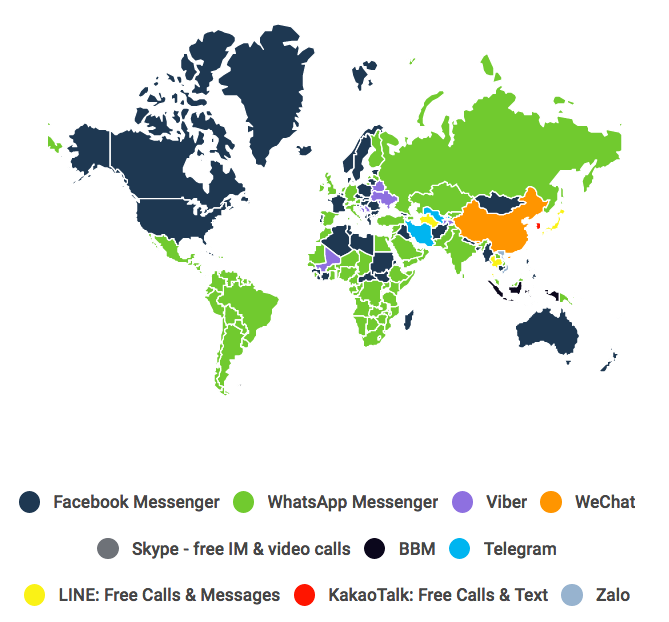
\includegraphics[width=0.7\textwidth]{images/similarweb-messenger-by-country.png}
	\caption{Most Popular Messaging App in Every Country\cite{similarweb}}
	\label{fig:similarweb}
\end{figure}

One important factor can be the geographical location of the target audience.
\\
As visible in figure \ref{fig:similarweb}, Facebook Messenger and WhatsApp are the global leading messengers,
and as previously mention the markets in China and Japan is dominated by WeChat and Line respectively,
but the data shows some lesser know trends; for example the Thai market is also dominated by Line
and in Iran, Telegram is the most popular messenger application.


\subsection{Cross-platform}
\label{crossplatform}

As with the creation of other kinds of software it is possible to release the same chatbot software for multiple target platforms. In similar ways to other platforms, the interaction of the software with the platform has to conform to the technical details and protocols of each target, the usage of platform-specific features has to be adapted individually and the user experience needs to be designed to fit each environment's expectations.
\\

There are also existing frameworks that allow developers to develop a chatbot once and release it to multiple platforms at the same time, without any modifications for the individual platforms.
\\
One such framework is API.ai by Google. As of writing they support 16 different integrations, including platforms such as Facebook Messenger, Skye and Slack\cite{apiai}. However, this platform is more than an adapter to different platforms. It's an complete solution to developing chatbots. API.ai comes with built-in support for natural language processing. A chatbot is already able to have basic conversations out of the box. The developer can train the bot about new topics by just providing example conversations while the framework handles all of the language parsing.
\\
Detected keywords and intends can be forwarded to be handled with custom logic; although for simple use cases this might not be necessary and a chatbot can be developed without writing a single line of code.
\\

Still, there are limits of what can be achieved with a platform like API.ai.
\\
First, intend parsing is, in the case if API.ai, currently limited to a finite list of topics. If a chatbot is handling topics from a domain unknown to API.ai, this solution is not sufficient anymore.
\\
Further, developers have no control over the applied machine learning and natural language processing algorithms.
There are no possibilities for customization, if the parsing results or the generated response do not match the requirements.
\\
Additionally, while API.ai currently supports 15 different languages, a chatbot is limited to the available languages.
If an new language needs to be supported, a lot of work might be necessary switching to a custom solution.
\\
Another issue to keep in mind is, that, while API.ai has support for many platform-specific features such as custom formats for message content and quick reply buttons, there are unique features of single platforms that are not supported and since the space is evolving at such rapid pace future extentions might not be available either.
\\
As last point it should be mentioned that, even though API.ai is at the moment free to use for everyone, they will very likely search for a sustainable business model in the near futre. This business model could be charging for the service or, being part of Google, simply collecting data, binding customers and gaining market share. Regardless which monetization strategy is chosen, as a developer one has to be aware that this is a non-controllable, external dependency.

\section{Classification}
\label{classification}


With the amount of messaging platforms opening up for chatbot development, companies have become interested in releasing their product for this new format and some developers created new products focusing solely on the chatbot market.
\\

Chatbot development is still a new market with a lot of changes happening all the time but there are some current trends in what companies are interested in creating. The direction might change soon in the future and there are probably still many undiscovered possibilities.
\\

\subsection{Categories}

One helpful classification of chatbots is categorizing them in terms of features they provide. The following categories are adapted from the article ``7 Types of Bots'' by \emph{Dotan Elharrar, a Product Manager at Microsoft AI \& Research}\cite{bottypes}.


\paragraph{Single-feature Chatbots}

A popular category of bots provide only one single feature. These bots are limited in functionality but simple to use. One example is a Facebook bot called Instant Translator\cite{instanttranslator}; in the beginning the user selects one language to translate to and all the bot does from there on is to translate all text it receives from the users language to the selected target language.


\paragraph{Proactive Chatbots}

This category are chatbots that push information to the user instead of answering questions in conversations. Hereby the user doesn't need to interact with the chatbot, but only uses it as service to receive information at certain times. One example would a service which sends the user a daily weather forcast. Another use-case is the Chatbot from the airline KLM\cite{klm}; a user can use the service to get updates and information about their flights delivered.


\paragraph{Group Chatbots}

There is a range of functionality chatbots can provide when they interact with a whole group of people instead of only a single user. These chatbots are limited to platforms which provide the necessary features to use chatbots in group conversations. A simple example for a Group Chatbot is called Roll\cite{venturebeat}; when sending a question to Roll the chatbots answers with one name of the members of the group.


\paragraph{Simplification Chatbots}

In a few cases chatbots are used to provide users with a simpler interface to complicated existing tasks which traditionally require the handling of a lot of bureaucracy. One example is a service called DoNotPay. It is advertised as "the world’s first robot lawyer"\cite{oreilly} and the service helps the user with simple legal problems, such as fighting a parking ticket.


\paragraph{Entertainment Chatbots}

One of the most popular kind of chatbots are still chatbots whose functionality consists only of having conversations with users. These services don't interact with other resources apart from the conversation itself. The previous described ELIZA belongs to this category.


\paragraph{Personal Assistants}

This category consists of chatbots that combine many different features and can be seen as platforms of their own. Siri and Alex, which have been mentioned earlier, belong to this category.


\paragraph{Optimization Chatbots}

Most companies are interested in chatbots in this category. The idea is to make an existing product more accessible by creating a chabot for users to connect to the product. By taking advantage of new platforms companies like to reduce friction for customers to use the product. The currently most obvious aspect of the chatbot platforms is the ease for users to access the products. Companies like to optimize the use of their product by making it available via the conversational interfaces of chatbots.
\\

\subsection{Products}

Use cases fitting this category can be found across many different industries. The article ``100 Best Bots For Brands \& Businesses''\cite{topbots} lists examples from different industries using chatbots to optimize access to their products. Products include beauty brands such as Sephora, consumer goods like Johnnie Walker, entertainment companies including Disney and Marvel, fashion brand such as H\&M, financial services like PayPal, food delivery from stores such as Pizza Hut, E-Commerce platforms including eBay, Traveling services such as Airbnb and Expedia, Airlines like Lufthansa and British Airways and many news outlets including Washington Post, New York Times, Forbes and BCC.
\\


As apparent from the engagement of many well established companies, brands are very interested in being present on messenger platforms.
\\

While there is big interest in targeting messaging platforms as a new market, the consumer engagement and the development efforts are nothing compared to established markets such as mobile applications or the web. Most of current products only provide limited features and are mostly created to connect customers to existing products.
\\

With increasing interest, engagement and, subsequently, financial investments the arise of more sophisticated products can be expected in the future.

\section{Promises}


As explained previously in \ref{presentday}, the interest in chatbots and conversational interfaces increased in recent time, because of the advancements made in the field of artificial intelligence and the popularity of messaging platforms, mobile devices, and personal assistants like Siri.
\\
The conditions are right to think about using the newly available possibilities, however, the question remaining is why we would want chatbots. What can chatbots achieve that existing solutions are not good at, both, from a user's point of view and looking at the interests companies have.
\\

From a user's point of view chatbots can be seen as a new interface to interact with computers.
Existing interfaces are not intuitive to humans. Using technology is something humans need to learn first.
With every new application one uses and every new website one visits there is a new interfaces to adapt to.
``Adjusting to a machine does not come naturally to us. With every app you need to learn how to use it. ... Conversations come naturally to us''\cite{techinasia}.
Conversation is a way of communicating humans already know how to use because they use it to interact with other humans.
If it is possible to use this communication technology to interact with machines, it should be really intuitive for humans to use it.
``The vision for a chatbot: get machines to respond to questions like a human being''\cite{techinasia}.
\\

Further, there is a trend in consumer behavior of ``outsourcing their "chores", such as driving, shopping, cleaning, food delivery, errands''\cite{chatbotbook} to companies that offer these services.
Service companies are not a new occurrence, however, in the past it took more effort to coordinate the usage of such services.
By using technology to automate many steps of the coordination process, not only the cost can be lowered, but also the friction for customers using a service is reduced significantly.
Managing and coordinating the usage of such services is a task conversational interfaces are particularly suited for because it is a scenario that profits especially from the simplicity and low friction that characterize conversational interfaces.
\\

Users can also profit from technical advantages of chatbots over to native applications and websites.
\\
Native applications need to be downloaded first which includes all resources and not just the ones we require at this moment.
Websites are a little slimmer and one only needs to download the resources required to load the current page.
But one page still contains not only content, but also layout information, styling, decorative images and in most cases also Javascript to run some additional logic in the web browser.
\\
The only thing a chatbots needs to download over the network is the content. Everything else is provided my the platform it is embedded in.
Compared to these existing solutions, ``a chatbot uses very low bandwidth''\cite{techinasia}, which can be an important advantage not only for the perceived responsiveness but especially in places where slow network connections are still common.
\\

Providing customers a more intuitive and more direct way of interacting with a company's product is already a compelling reason for a company to be interested in the new platforms, but there are additional benefits companies can draw from conversational interfaces, which are not perceivable for the users.
\\

First, ``the cost of developing a chatbot is one-third of what is required in developing a mobile app''\cite{techinasia}. This might not be the case for every single product but in general, creating a chatbot is less work than creating a mobile application, because there is no custom design required nor  is it necessary to write code for the logic controlling the user interface.
\\

Next, ``Chat apps also have higher retention and usage rates than most mobile apps''\cite{businessinsider}. Since chatbots are part of a chat application they can take advantage of being where the attention of mobile phone users already is. A chatbot can therefore potentially gain more user engagement than a competing website or mobile application.

Another aspect of the flexible nature of using natural language as an interface is that ``chatbots are able to gain invaluable data and insights on user behavior''\cite{drum}, because firstly, users have the freedom to send any kind of information and feedback and secondly, being in the context of a conversation people tend to be more talkative than they would be in a more formal environment.
Especially for companies such as media outlets or retailers being able to further profile users can be a useful assistance in tailoring personal experiences for users and targeting them with individual offers.
\\
Additional context and user data is also available on the platform itself; when interacting with a user via a chatbot on the Facebook Messenger platform all public information of the user's Facebook profile is also available for the company to user for further personalization.
\\

Lastly, the most fundamental reasons for a company to be interested in chatbots as a platform are the before mentioned popularity and ubiquity of messenger applications.
``The question brands and publishers now face is how to engage with these private social network users''\cite{drum}.
When the attention of users is shifting away from not only non-digital media but also away from other mobile applications, including traditional social networks, companies need to find a way to reach users at the place they spend most of their time at.


% APIs ``can be accessed from computers to complete real world tasks''\cite{chatbotbook}
% Already covered in previous chapter:
%``After nearly a decade of explosive growth, mobile apps have largely stopped growing''\cite{chatbotbook}
%``Social and messaging apps emerge as big winners''\cite{chatbotbook}
% ``Artificial Intelligence has gotten a lot better''\cite{chatbotbook}
% Graphic titled ``Messaging Apps Have Surpassed Social Networks''\cite{businessinsider}

\chapter{Development}


To not only understand possible applications of chatbots but also understand what the practical development of a chatbot looks like this chapter guides through the development of an example chatbot.
\\

To start with, an appropriate application needs to be chosen and specified in its requirements.
Before starting with the implementation possible usage scenarios need to be defined and matching user stories will be created.
\\
When all requirements are set, the appropriate platforms, tooling and solutions can be selected.
After all preparations are done the technical implementation will take please.
It is followed by any analysis of complications and a comparison to other possible solutions.


\section{Choosing a Practical Example}

Before thinking about implementation details a suitable application for a chatbot needs to be selected.
\\
As illustrated earlier, chatbots can be used to cater a wide variety of applications.

Since this example application should be a suitable demonstration of the different aspects of developing chatbots,
it should not be too simplistic in scope.
An appropriate example covers more than one of the product categories described in section \ref{classification},
while being, at the same time, not too technical challenging in a problem domain which is not a specific to chatbot development.
\\
A service, that accepts image files and returns the same picture with a filter applied, might be an interesting and entertaining use case for a chatbot, however, it would not be an adequate example to give a general introduction to chatbot development since, even though it would a technical interesting task to solve regarding image processing, it would not illustrated much technical details in the domain of chatbot development.
\\

The here selected example application is a system for individual language studying.
\\
While this idea arises from a personal need for such a system and an observed shortage in the functionalities existing solutions provide,
this application also fulfills the stated requirements of a suitable example application.
\\

The language studying chatbot covers multiple of the categories defined in the section \ref{classification}.
\\
Mainly it's a simplification chatbot simplifying the task of language studying,
but the chatbot can also be classified as a proactive chatbot because it uses proactive features to notify the user when it is time for studying.
\\

Although there is a necessity to understand parts of the problem domain of language studying,
the required domain-specific knowledge is minimal and the main communication medium remains text-based.
\\

The idea is to build a system independent from existing learning resources, that users can use to study their own vocabulary.
Since there is no need to focus on content for specific languages, the main focus remains the implementation of the chatbot features.
\\
In short, a user is able to input new vocabulary; then the system tests the user's knowledge in appropriate learning intervals.

\section{Existing Solutions}
\label{existing}

When starting a new projects it is helpful to research for existing solutions that might solve the same problem.
\\
There is already a variety of existing software applications for language studying, which have very different use cases and solve different problems.

One significant separation is between software that includes content and software the user can customize to study personal content.
\\

The first segment is the most prominent. This software is intended to enable people to self-study language and, at least partially, replace physical language courses.
\\
A main reason for the prominence of this segment can be attributed to the ability to sell content.
Professionally curating a language course curriculum requires teaching expertise and is a lot of effort, and therefore content remains expensive, not only in software but also in the form of physical textbooks.
\\
One popular example from this segment is Duolingo. ``Duolingo has courses in a handful of languages.... The courses are structured in a way like games as well - you earn skill points as you complete lessons''\cite{lifehacker}.
\\
Interestingly, Duolingo recently released a chatbot\cite{topbots2} as part of their iPhone application which enables the user to have a written conversation about certain topics with a chatbot and to thereby learn the appropriate phrases for the given scenario. Although the topic and possible phrases are restricted in each scenario, this is a first example of how chatbots can be used for language studying.

% TODO: think about metioning Mondly and Eggbun here
% https://blog.mondlylanguages.com/2016/08/25/mondly-chatbot-press-release/
% http://www.tofugu.com/japanese/japanese-learning-resources-april-2017/#eggbun


The second segment consists of software which doesn't not provide users a guideline what to study but is instead intended to support users studying their own content.
\\
Most of the software that can be found in this segment is a variation of the attempt to bring traditional flashcards to digital media.
\\
One of the most established software in this segment is Anki\cite{lifehacker}, which exists for more than ten years already and provides a flexible, but also rather complex, interface to create a various kinds of studying material.
\\
Another more recent competitor is Memrise, where users get a more intuitive interface, which also includes several gamification\footnote{The Oxford Dictionaries describe gamification as ``the application of typical elements of game playing (e.g. point scoring, competition with others, rules of play) to other areas of activity''\cite{oxfordgamification}} features to make the studying process more appealing.
\\
Both mentioned products are not restricted to a field of study and users are able to add their own content. Furthermore both products also offer mechanisms for users to share content with each other, which allows users to reuse what other users created instead.
\\

For the here planned chatbot example the second segment is more fitting, since there are no resources in the current context to curate professional content.
The following implementation is an attempt at creating a software product with a conversational text interface that is in its use cases similar to products like Anki and Duolingo while using the unique features chatbots as a medium provide compared to the here mentioned products.

\section{Definition of Use Cases}

Building on the analysis of existing solutions in \ref{existing}, features for the chatbot need to be specified.
\\
An effective method for gathering crucial features is by finding potential users
and creating usage scenarios for their individual needs.
\\

To apply this method, the fundamental problem the application is solving needs to be defined.
\\
The issue this chatbot is trying to help with is the study of individual vocabulary.
The goal is not to provide studying material in a way a language course or a textbook does,
but instead to complement these resources with a tool to study new vocabulary and phrases the learner picked up
while studying or in a different situation in every day life.
\\


\subsection{User Stories}

The following are two individuals that might possibly use the chatbot and both of them profit from it in different ways.
\\

Clara is a 22 years old American.
She moved to New York City to go to University.
Currently she's in the last year for her Bachelor degree in economic.
In University she signed up for an evening class in Mandarin.
She uses Facebook Messenger every day to talk to her friends and when a friend sent her a link
she found the chatbot.
For her the most difficult part of the studies is to write hànzì, the Chinese characters.
Now Clara uses the chatbot to write down vocabulary in hànzì during her class,
and at home she revises the new characters by going through them using the chatbot and writing the characters
down on paper.
\\

Pierre is 29 years and born in Bordaux in France.
He studied computer science.
A year ago he moved to Berlin where he found a job at a startup.
At work everyone all communication is happening in English since the team consists of people from all around the globe.
Because Pierre is not a native English speaker, he picks up new words at work almost every single day.
Since moving to Berlin Pierre also made a few German friends and he tries to pick up new words they teach him
and he also tries to remember things he sees in the supermarket.
He found the chatbot on a news website for technology products,
and since then whenever Pierre learns a new word he gets his phone from his pocket and adds the word to the chatbot.
Since the chatbot has no restrictions on what to learn, Pierre uses it to save both, German and English, vocabulary in one place.
Pierre's daily commute from and to work takes him 40 minutes each.
Now he takes advantage of this time by taking out his phone and reviewing new vocabulary he picked up the previews days.
\\


\subsection{Features}

The above defined user stories can be used to extract all necessary features.
\\

First, a user needs to be able to add new vocabulary.
\\
There should not be any restrictions on what to add
and vocabulary should not be limited to single words because in many cases it is more useful
to add whole phrases instead.
\\
Each vocabulary consists of the phrase the user is trying to remember
and an explanation to help the user understand what the phrase means.
\\

Next, users need a way to revise vocabulary.
\\
There should be two possible modes for revising;
one version where users can decide on their own when to go to the next phrase
and if they remembered the phrase correctly,
and a second way whereby users type out the phrase right in the messenger application.
\\
In each case the system should keep track of wheather the user new the correct solution or not.

\\
Last, it is necessary to have a means of deciding what to study next.
\\
A user should not be required to think about what to review or even when it is the right to review vocabulary.
The chatbot needs a system to decide the review time for each vocabulary,
and ideally the user is notified when vocabulary is ready to be reviewed by sending a message to the user.
\\


These three main features can be seen as a sufficient minimal viable product, MVP, for this chatbot.
\\
For demonstration purposes it is desired to keep the product as simple as possible.
\\
The knowledge that can be taken from making decisions about the implementation and walking through the process of creating the chatbot,
is mostly independent from this particular product and can be applied to the development of similar chatbot products.


\section{Setup and Requirements}

After knowing the features the chatbot should support,
technical requirements can be extracted
and appropriate technology can be chosen for the implementation.


\subsection{Communication}

As discussed in \ref{communication} on page \pageref{communication},
there are two fundamental ways for communicating with a user,
interface elements and natural language.
\\

Since the previous defined features for the minimal viable product of the example chatbot are so basic,
there are not many options required and everything can be represented in an unambitious interface.
\\

The precise actions necessary to be defined are shown in the next section.
For now it should be sufficient to know that all of them can be represented as predefined actions.
\\
However guiding the user with interface elements instead of natural language
does not imply that natural language can not be used complimentary.
\\
Quite the contrary, the example chatbot is only possible by analyzing user input;
when adding new vocabulary phrases and their explanations need to be captured,
and likewise the user's guess needs to be evaluated when studying.
\\

The implementation of this chatbot demonstrates the complementing use of interface elements and natural language side by side.
\\

By relying only on simple input parsing and no advanced artificial intelligence based natural language processing techniques,
a major source of complexity of chatbot development can be avoided.
\\
While these are useful techniques that enable previous impossible use cases,
they are not necessary to explore the fundamentals and paradigms of chatbot development.
\\

\subsection{Platform}

An important question to answer when development a chatbot is which platform to target.
As shown in \ref{platforms} on page \pageref{platforms} there are many possible target platforms
and some are fundamentally different.
\\

Deciding for a voice-based platform like Alexa, or for SMS or a messenger platform has consequences
for all other decisions.
\\
For the case of the example chatbot, while possible, a voice-based interface is rather unsuitable since
users should be able to control the precise spelling of the vocabulary
and further, there is currently no voice-based platform available
that supports multiple languages simultaneously.
\\

SMS communication is better suited for scenarios that only need to send a low number of messages,
since, although the prices are pretty low, there are costs for sending text messages.
\\
As of writing, Twilio charges \$0.0075 for receiving and \$0.085 for sending per message when using their Global Short Message Service API in Germany\cite{twilio}.
\\
Supposed the chatbot has 1000 active users that all study 100 phrases daily,
the costs would accumulate to \$277500 of monthly expenses\footnote{1000\times100\times30\times(0.085+0.0075)=277500}.
These prices are affordable if a company is selling airplane and send tickets directly to users' phones,
but in other scenarios another messaging platform is more suited.
\\

By choosing a messaging application as target platform, there are no monthly costs to be taken care of.
Additionally there are further interface elements for interaction available than only plain text.
But there are many major existing messaging applications and the choice can be difficult.
As we saw earlier, different platforms have geographically different target markets.
If a chatbot targets the Chinese Market WeChat would be the obvious platform to choose;
likewise Japan would be targeted by using Line.
\\
In North America and Europe Facebook Messenger and Facebook's WhatsApp are currently the leading platforms.
Since as of writing WhatsApp does not provide a publicly available API, Facebook Messenger is the biggest platform one can target.
\\
By creating the first version of the example chatbot with English as an interface language,
the target markets are mainly North America, Europe and Australia and therefore Facebook Messenger would be a natural fit as target platform.
\\

As mentioned in \ref{crossplatform} on page \pageref{crossplatform}, there are also solutions to create chatbots using a framework which allows to release the chatbot to multiple platforms at the same time, but as previously noted such a framework also has drawbacks.
\\
With the limitations in mind and to keep the example as simple as possible,
it will be implemented for a single platform without abstracting the process by using third-party frameworks.
\\

Facebook Messenger is a fitting platform not only due to popularity,
but also because it offers mechanisms for interacting with chatbots via interface elements,
which will be used in the next chapter to display action buttons in the user interface.
\\


\subsubsection{Integration}

The development of a chatbot for Facebook Messenger is similar to most other platforms.
\\
When creating and configurating a chatbot, the developer registers a webhook URL.
``The concept of a WebHook is simple. A WebHook is an HTTP callback: an HTTP POST that occurs when something happens; a simple event-notification via HTTP POST.''\cite{webhook}
\\
After the setup is done,
Facebook will now send an HTTP POST request to the registered URL containing event information for every message a user sends to the chatbot.
This way the developer has complete control over how to handle each message on any machine that is reachable via a public URL.


\subsection{Server}

At this point that the interaction with the platform is decided, the application can be created on a custom server,
and it has to be decided to structure the application running on this server.


\subsubsection{Programming Language}

Since all interaction with the chatbot platform happens via HTTP,
there is no restriction on which programming language to use as long as it can be executed through a web server.
Chatbots can be written in any programming language.
\\
Depending on the specific application, different programming languages are better suited than others though.
\\

In the example case there are not any specific technology requirements.
\\
However, to be able to send notification messages to users when their studies are ready,
the system requires a way to schedule timers for the notifications.
The timers need to be lightweight enough to be re-scheduled for every user activity,
that can affect the time the notification is scheduled for.
\\
Single-threaded programming languages, such as Python, Ruby or PHP,
mostly use the pattern of using a separate worker process to handle scheduled jobs,
but in this case there would need to be another process for each user
just waiting until it is time to send notifications to the specific user.
\\
Another way to handle this in single-threaded programming languages is by using a system for \emph{asynchronous, evented I/O},
such as the \emph{asyncio} module for Python\cite{asyncio} or the Node.js JavaScript runtime\cite{nodejs}.
\\

The example chatbot is created with the Go programming language\cite{golang}.
\\
Go is a multi-threaded language which allows for taking advantage of all available CPUs
on a machine without the overhead of creating new processes.
\\
It is well suited for scheduling notifications and further Go has a robust web server in the standard library which can be exposed to the public Internet without a proxy server, that is common with the previous mentioned programming languages.
By making use of this there is less parts to take care of and the example can be a simple and self-contained application.
\\


\subsubsection{Data Storage}

Some applications do not store any data locally, but only process requests and send out replies.
\\
In the example case data needs to be stored and it should be stored locally on the same machine
to keep the application as contained and simple as possible.
\\

Since a user can save new vocabulary,
there needs to be a way to store information for each user.
\\
For the studying itself, further information has to be stored.
It is necessary to keep track of correct and incorrect guesses the user does while studying
and to decide when to study next, the time of the last study needs to be tracked too.
\\

To send notification additional information has to be stored.
It is necessary to know when the user was last active and if the user saw the last notification,
since notifications should only be send when the user is not already active at this moment
and when the user has not seen the last notification yet, no new one has to be sent either.
\\

All of the information required to be stored is always focused on a user.
Users can never share information with each other.
There are no complex relations between data.
\\
Without relational data there is not much use of features that relational databases such as MySQL or PostgreSQL provide;
a simple key-value store can be sufficient for storing this data instead.
\\
The example uses an embedded key-value store called Bolt\cite{boltdb}.
\\
No separate process is needed for the database and data is saved on disk in a single file.



This implementation and technical decisions are the base for the following description of the chatbot implementation.

\section{Feature Implementation}
\label{implementation}

\begin{wrapfigure}{O}{0.3\textwidth}
  \centering
  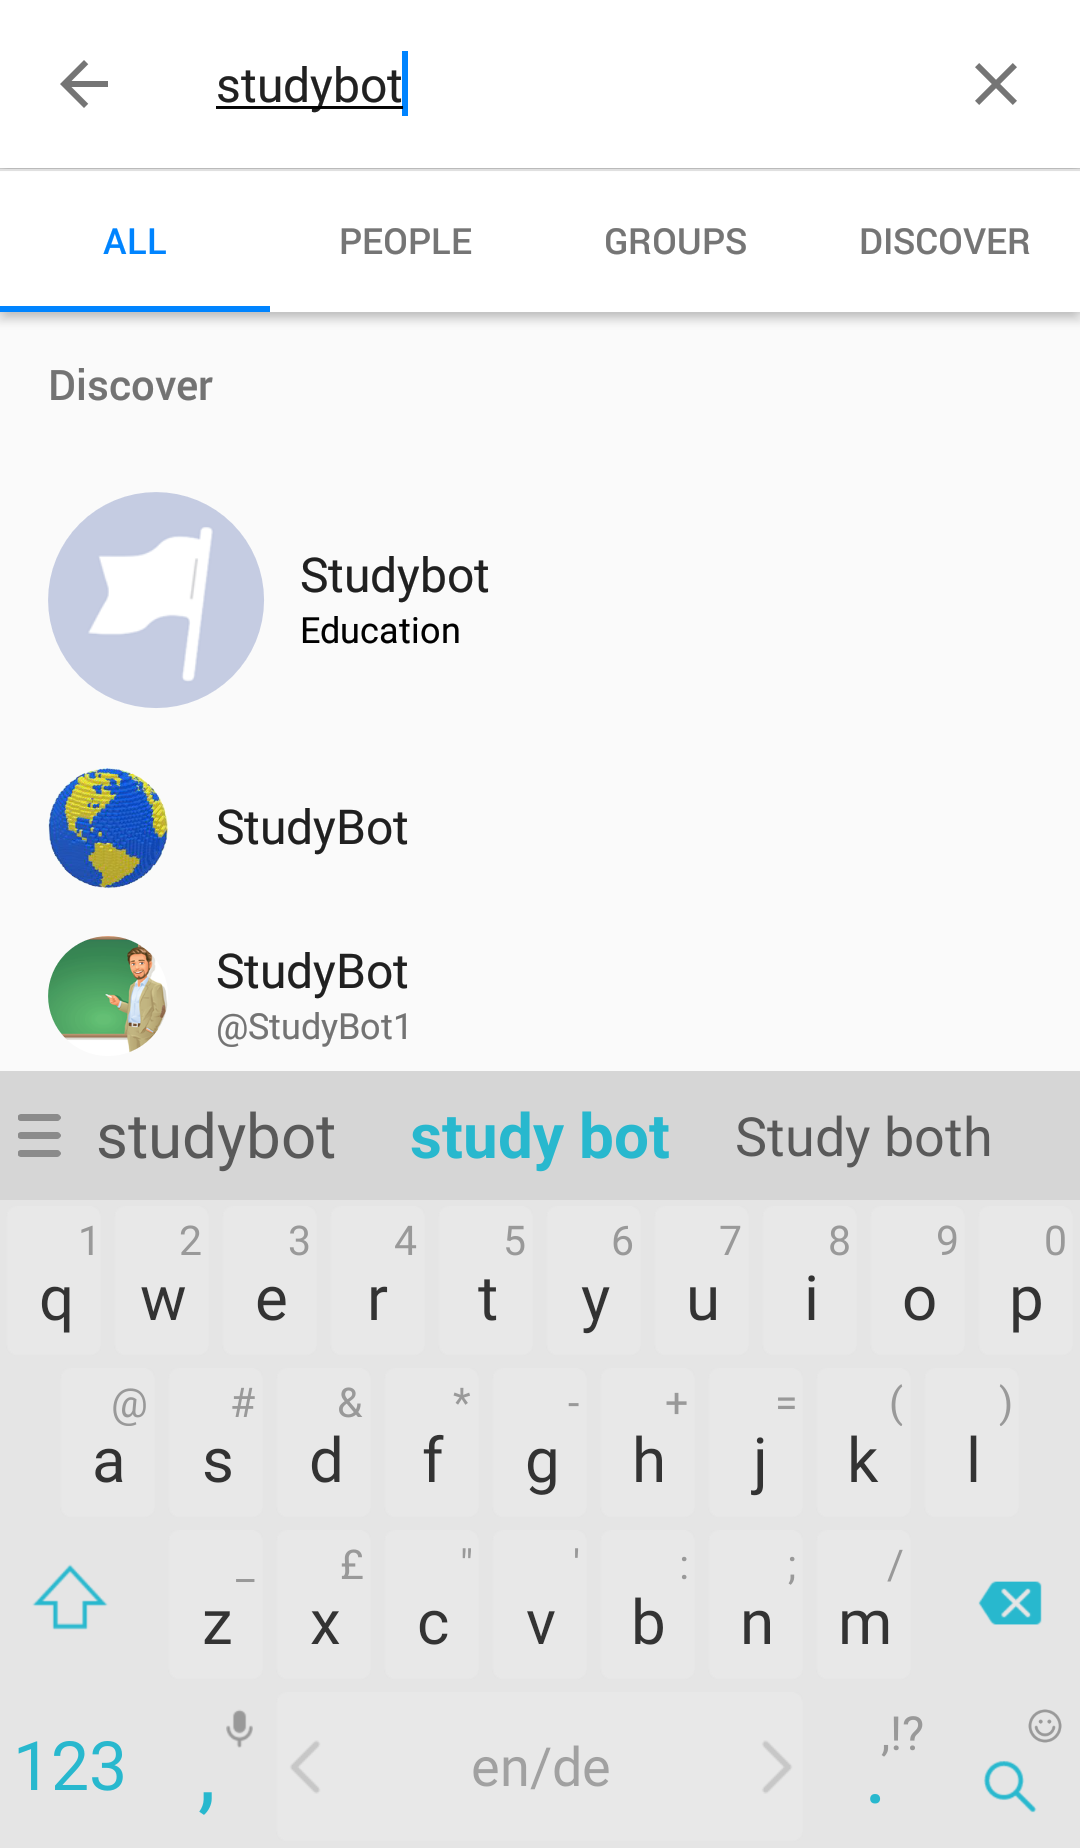
\includegraphics[width=0.28\textwidth]{images/interface/01-search.png}
	\caption{Search}
	\label{fig:01-search}
\end{wrapfigure}

At this point it is defined what the example chatbot is able to do,
and which technologies are used for its implementation.
\\

Before looking at the implemenation,
the usage of the chatbot is shown from a user's point of view.
\\
The following is a presentation of how this chatbot is used.
\\

Facebook Page and a Facebook Messenger bot have been created under the name \emph{Studybot}.
\\
By not publishing the Facebook Page, also the chatbot remains only accessible for administrators of the Facebook Page.
\\

The demonstration uses the Messenger Android application,
but Messenger bots can also be accesses through applications on other platforms
or using the web version of Facebook.
\\

When using the Messenger application as administror,
the bot can be found by using the search as shown in figure \ref{fig:01-search}.
\\

\begin{wrapfigure}{O}{0.3\textwidth}
  \centering
  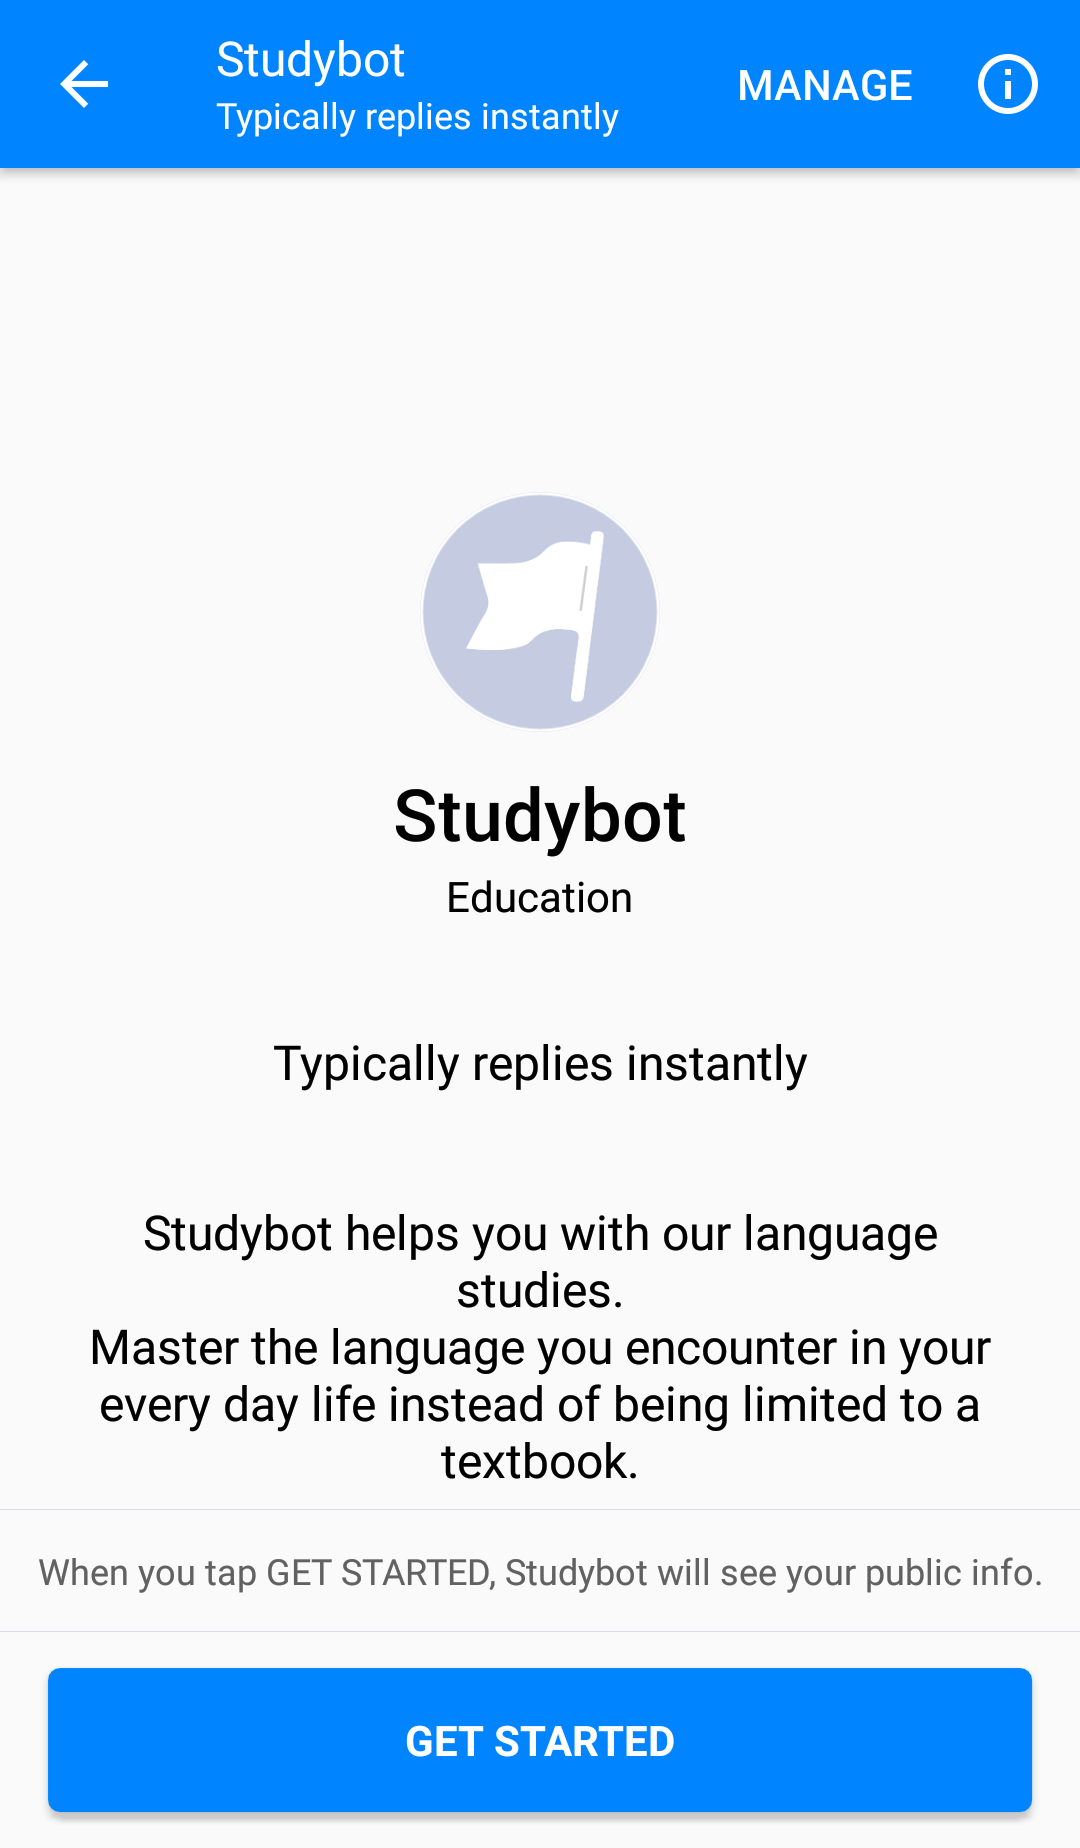
\includegraphics[width=0.28\textwidth]{images/interface/02-getstarted.png}
	\caption{Get Started Screen}
	\label{fig:02-getstarted}
\end{wrapfigure}

After navigating to the chatbot,
a description of the bot becomes visible.
This can be seen in figure \ref{fig:02-getstarted}.
\\
This view contains the profile image of the Facebook Page the chatbot belongs to,
the category the Facebook Page is part of,
and a text describing the functionality of the chatbot,
whereby all of these elements can be defined by the developer of the chatbot.
\\
A button labeled \textbf{Get Started} is displayed at the bottom of the view.
\\

\begin{figure}[h]
  \centering
  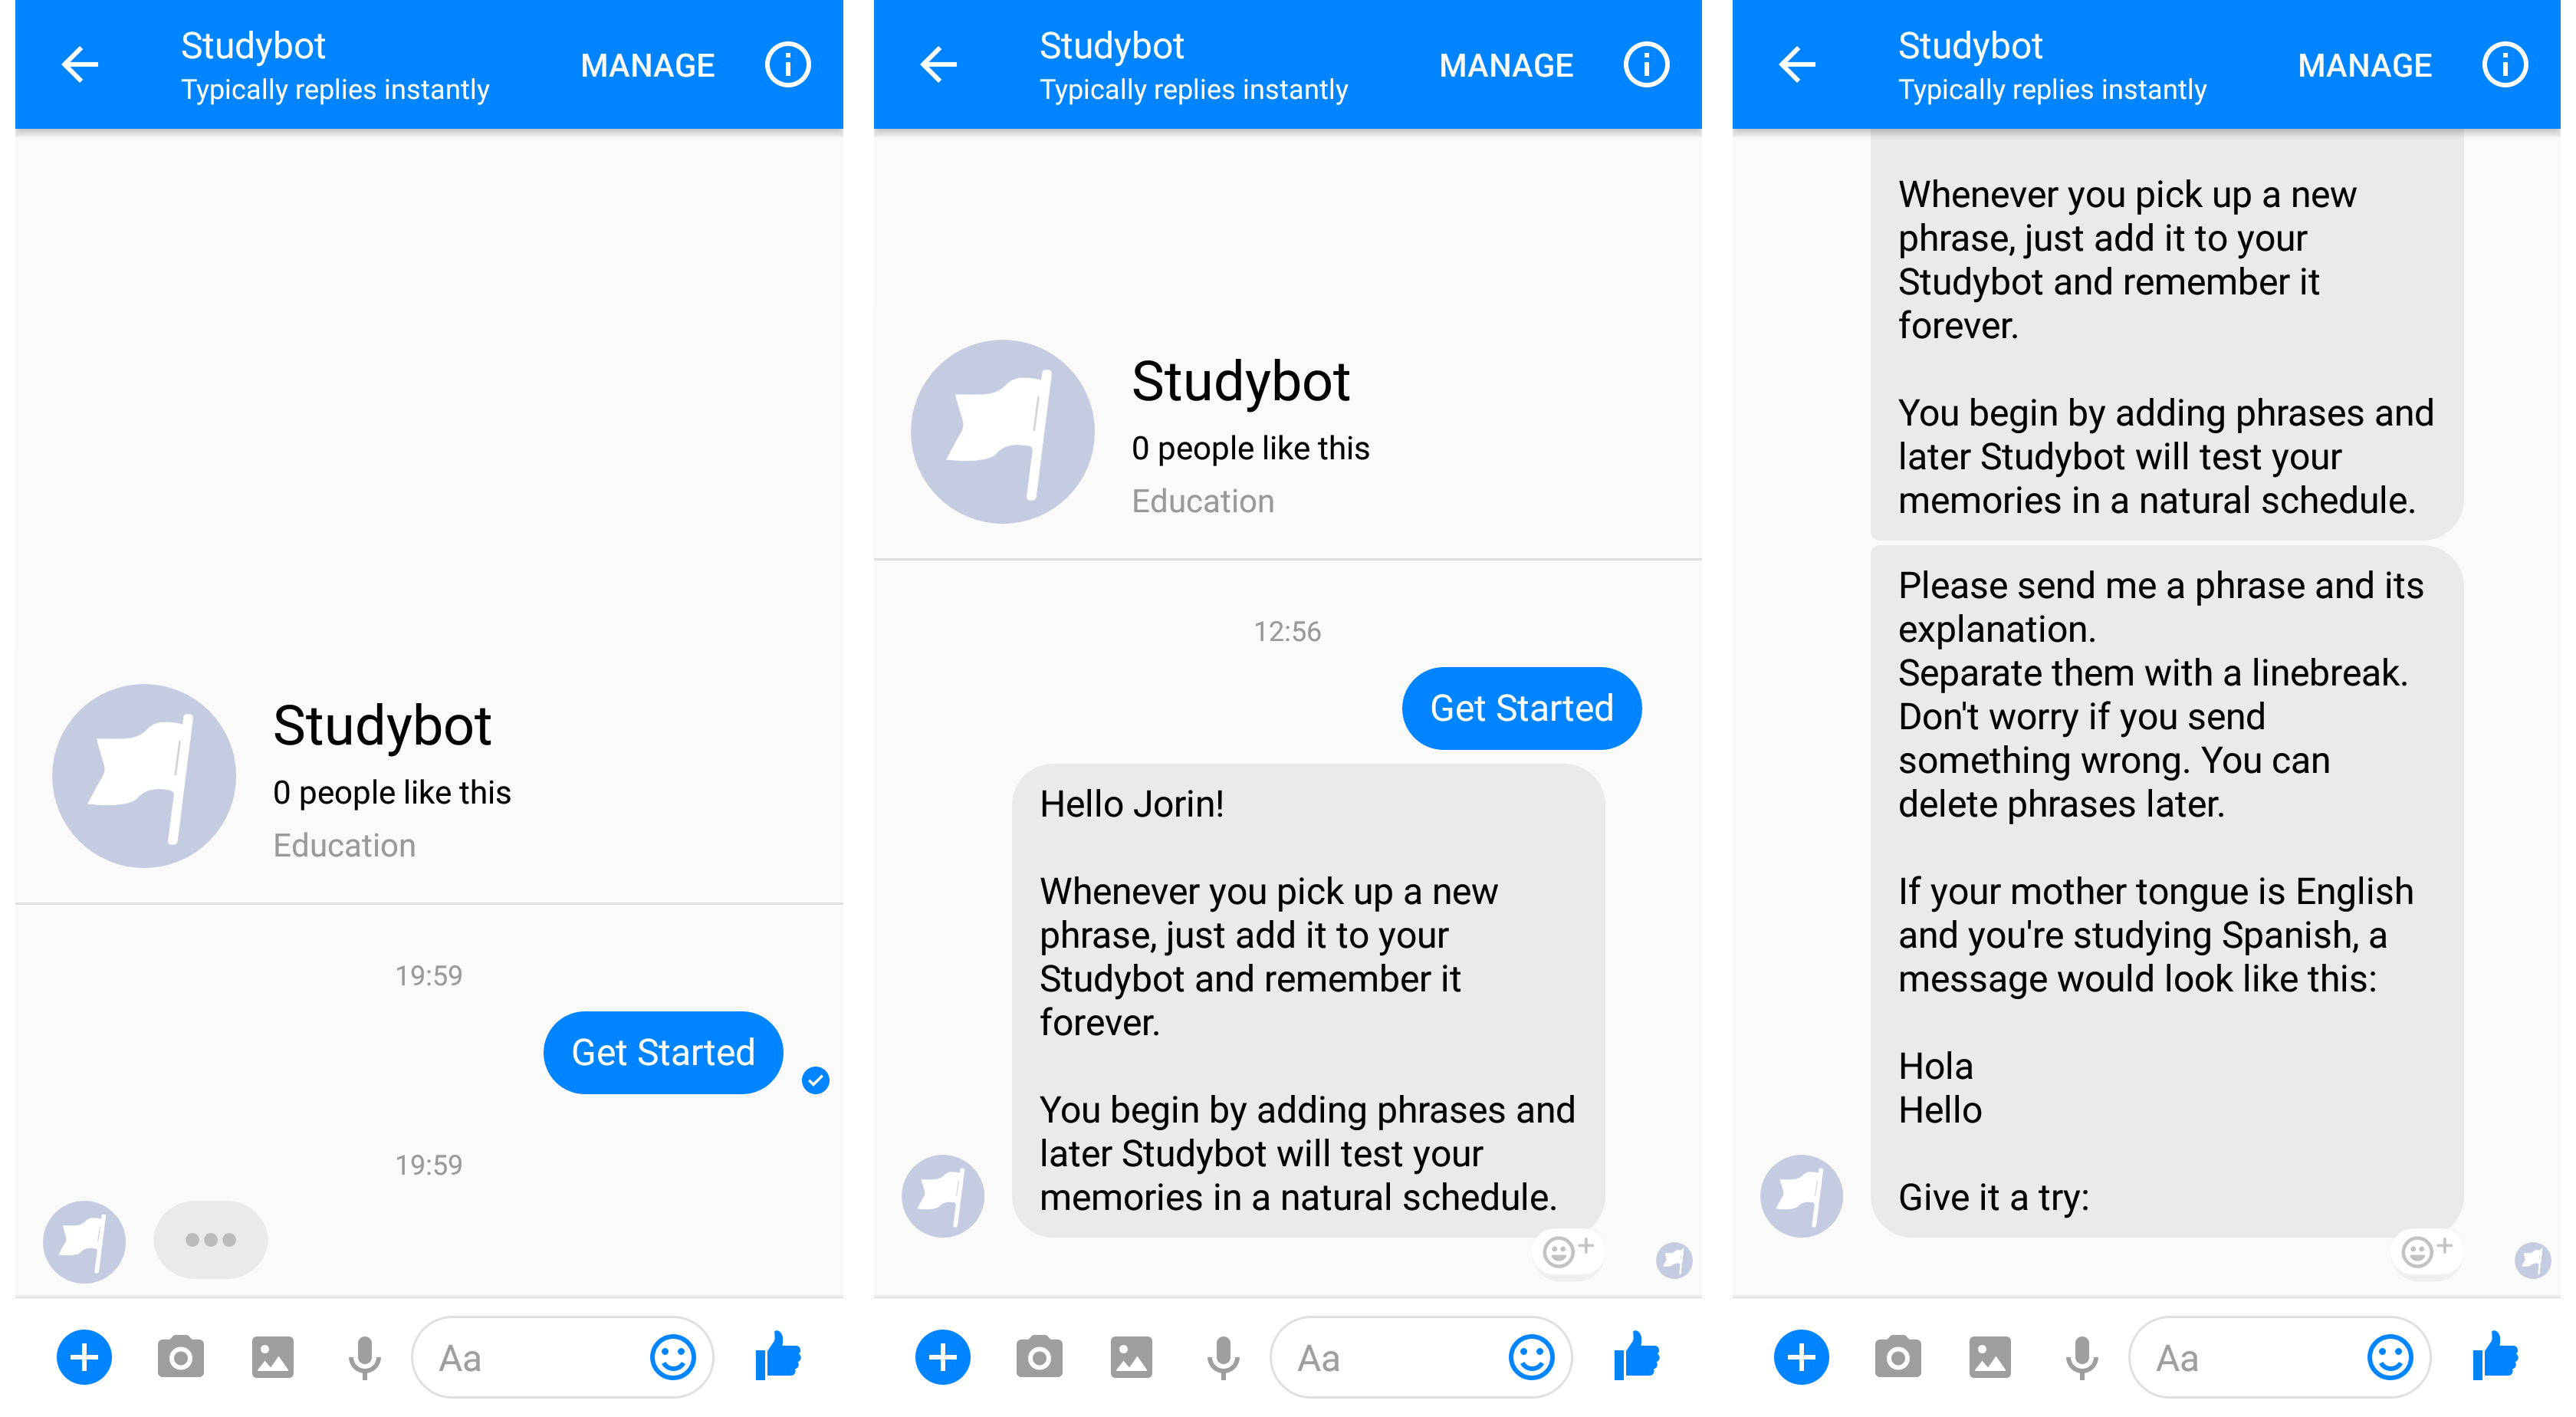
\includegraphics[width=0.9\textwidth]{images/interface/03-welcome.png}
	\caption{Messages introducing Studybot}
	\label{fig:03-welcome}
\end{figure}

When pressing the \textbf{Get Started} button, a message is sent to the chatbot,
and as indicated by the \emph{dots} visible in figure \ref{fig:03-welcome} in the left image,
the chatbot is active and about to send a reply.
\\
In normal conversations the \emph{dots} are used to indicated when a user is typing text.
\\
For chatbots the \emph{dots} indicated that the chatbot received the message and is crafting a reply.
\\

The image in the middle of figure \ref{fig:03-welcome} shows the first message sent to users;
users are greeted using their first name to create a more personal feeling atmosphere.
The greeting is followed by a two sentence long explanation of what this chatbot is doing.
\\
When working with text as a medium it is especially critical to focus only on the most important information;
with graphical elements and images users can perceive an impression with a single glace,
but to perceive the meaning of text the user needs to read word by word.
\\
Since in most scenarios the time users are willing to invest in understanding a product is limited,
every word in a text has to be selected carefully.
\\

It can be seen in the image on the right of figure \ref{fig:03-welcome} that a second message is sent to the user.
\\
The second message is delivered 5 seconds later that the first one to not overwhelm the users with too much information at once
by putting a \emph{wall of text} on their screen.
\\
This message contains instruction for the first step of using the application.
\\
The instructions are additionally illustrated by providing an example for a message in the expected format.
\\

\begin{figure}[h]
  \centering
  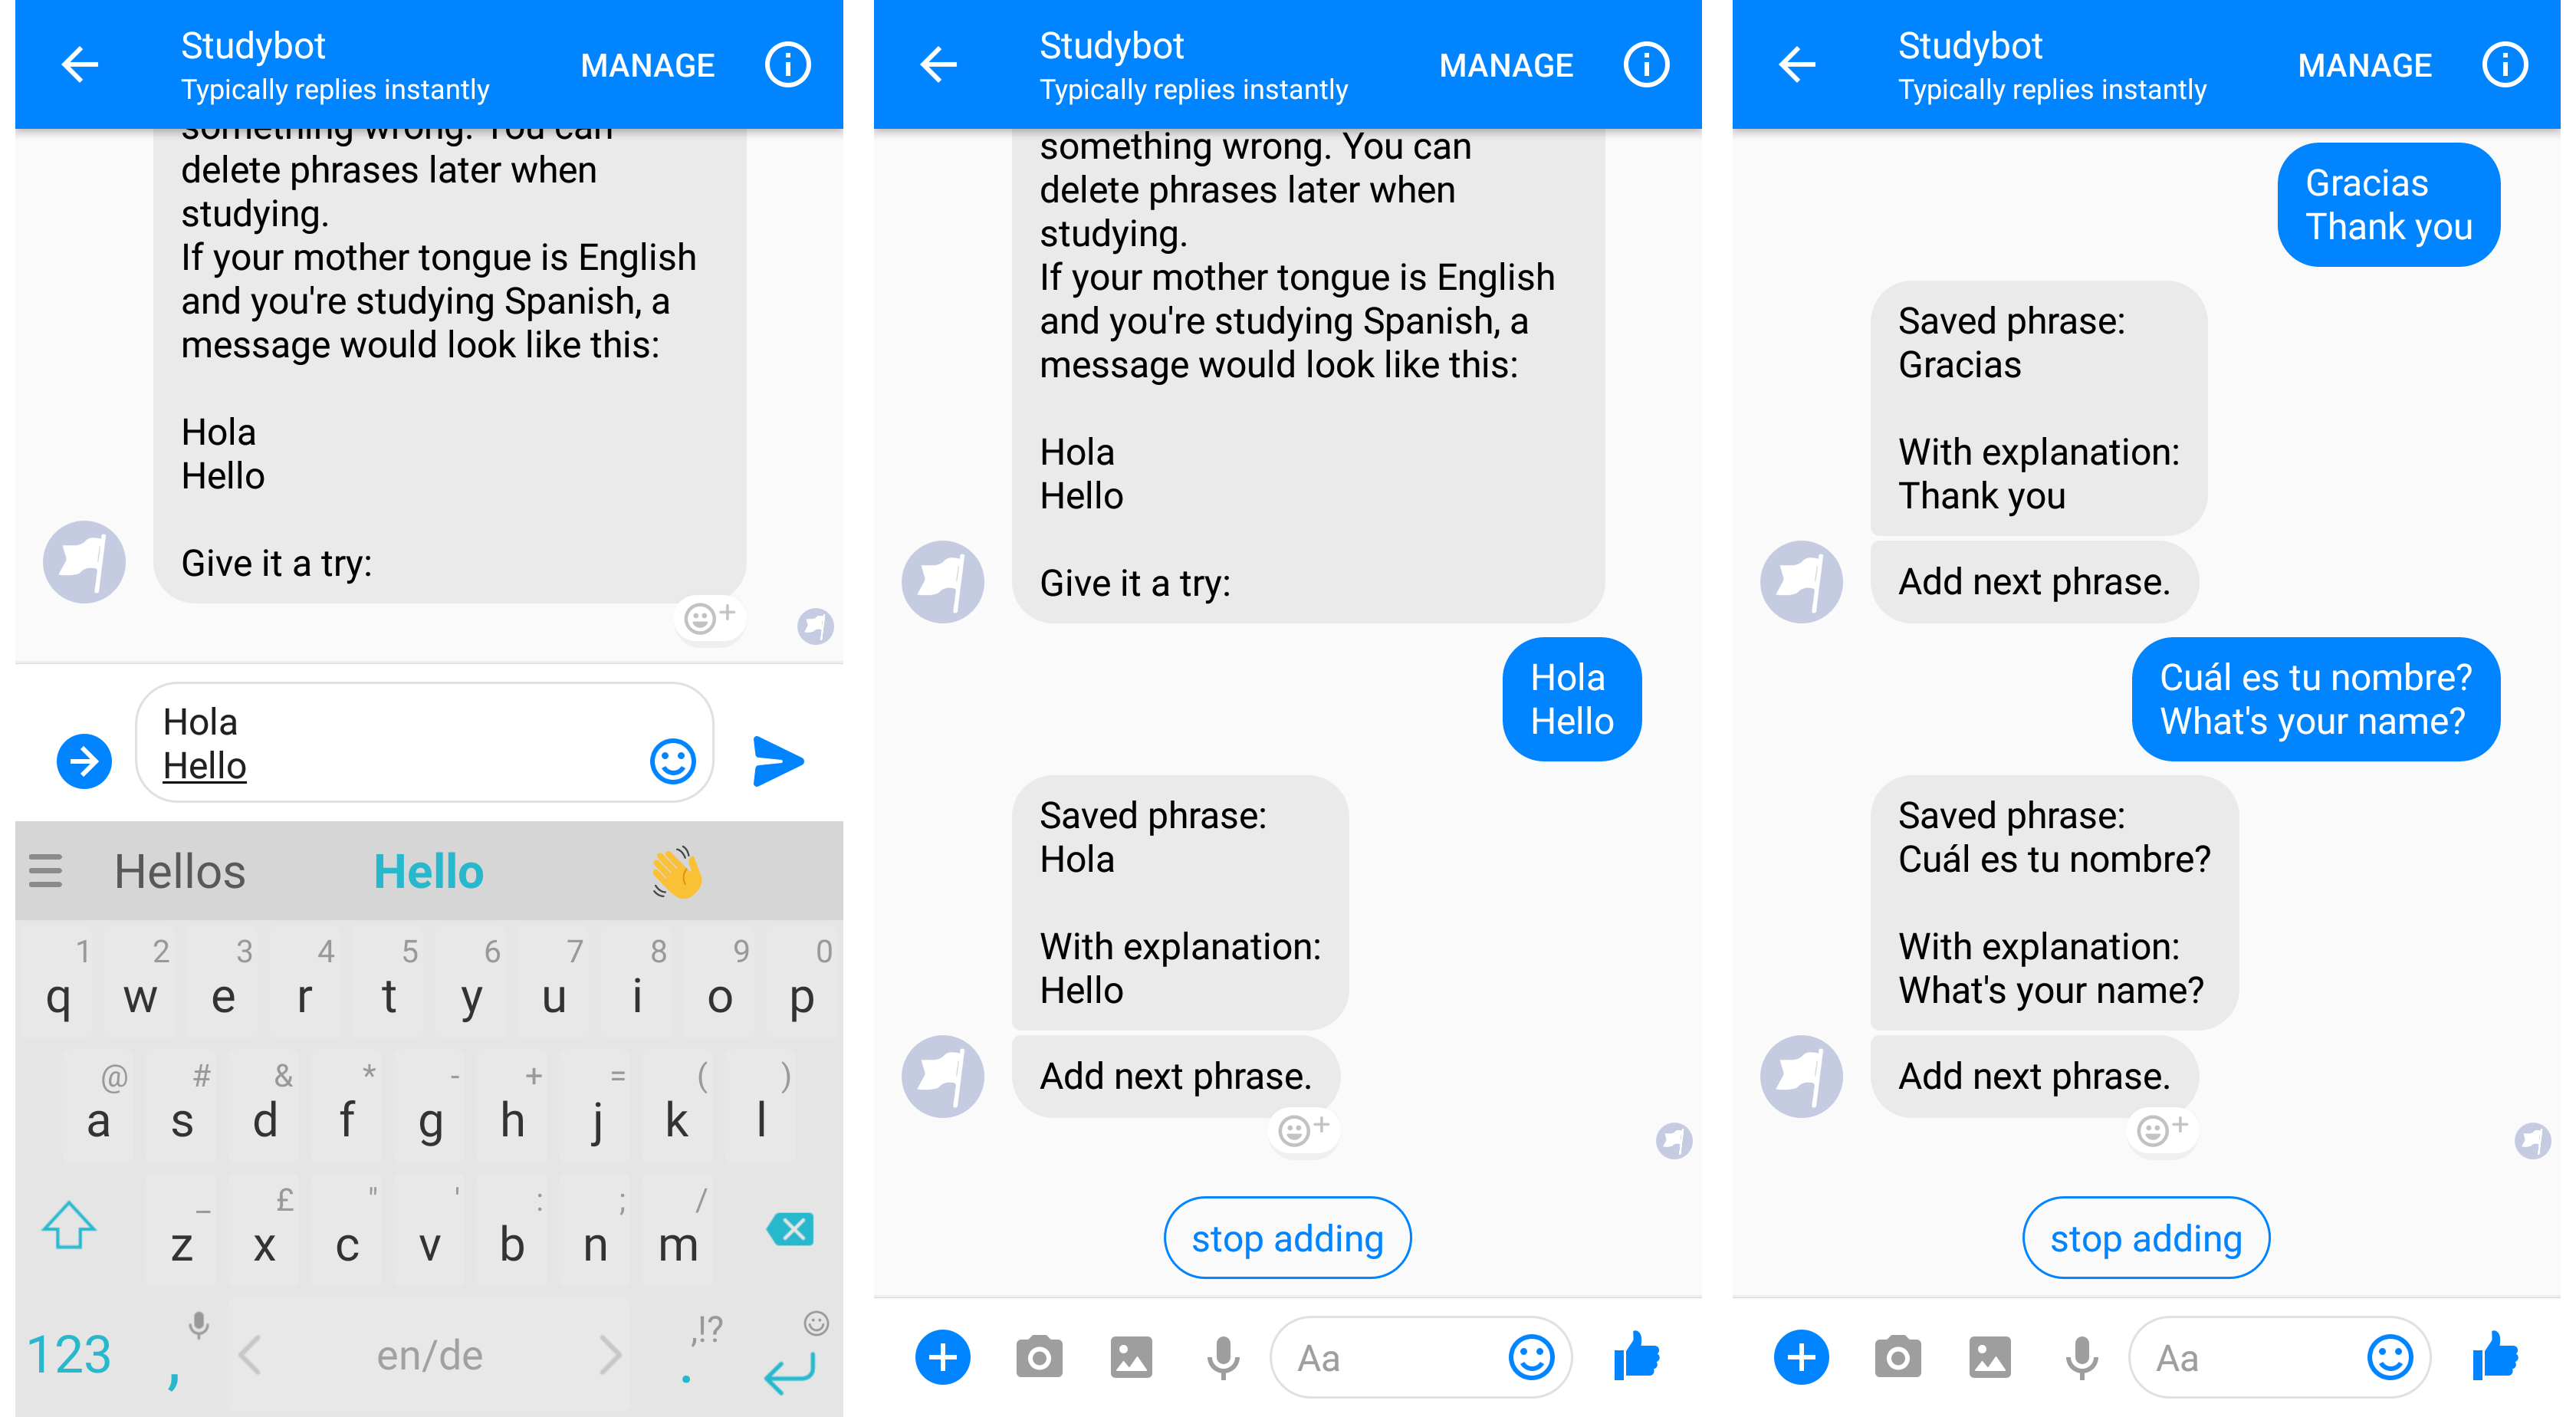
\includegraphics[width=0.9\textwidth]{images/interface/04-add.png}
	\caption{Adding three phrases}
	\label{fig:04-add}
\end{figure}

At this point the user needs to interact with the chatbot.
\\
Figure \ref{fig:04-add} shows how a user adds phrases to Studybot;
when typing a phrase, users first types the phrase in a foreign language they like to study,
then the \emph{return} or \emph{enter} key on the keyboard has to be used to insert a \emph{line-break},
and the next line contains an explanation for the preceding phrase.
\\
After the phrase is sent to the chatbot,
a confirmation message is displayed to keep the user updated about the current state of the system.
\\
This is followed by another message prompting the user to add more words.
\\
For a chatbot it is critical to always keep the user informed about the next expected action,
therefore a message should most of the time end with a prompt for a certain input or action.
\\

The image in the middle of figure \ref{fig:04-add} shows that this is the first point of the conversation,
that in addition to being able to type a reply, a button is displayed at the bottom of the messages,
which the user can use as an alternative way for interacting with the chatbot.
\\

\begin{wrapfigure}{O}{0.3\textwidth}
  \centering
  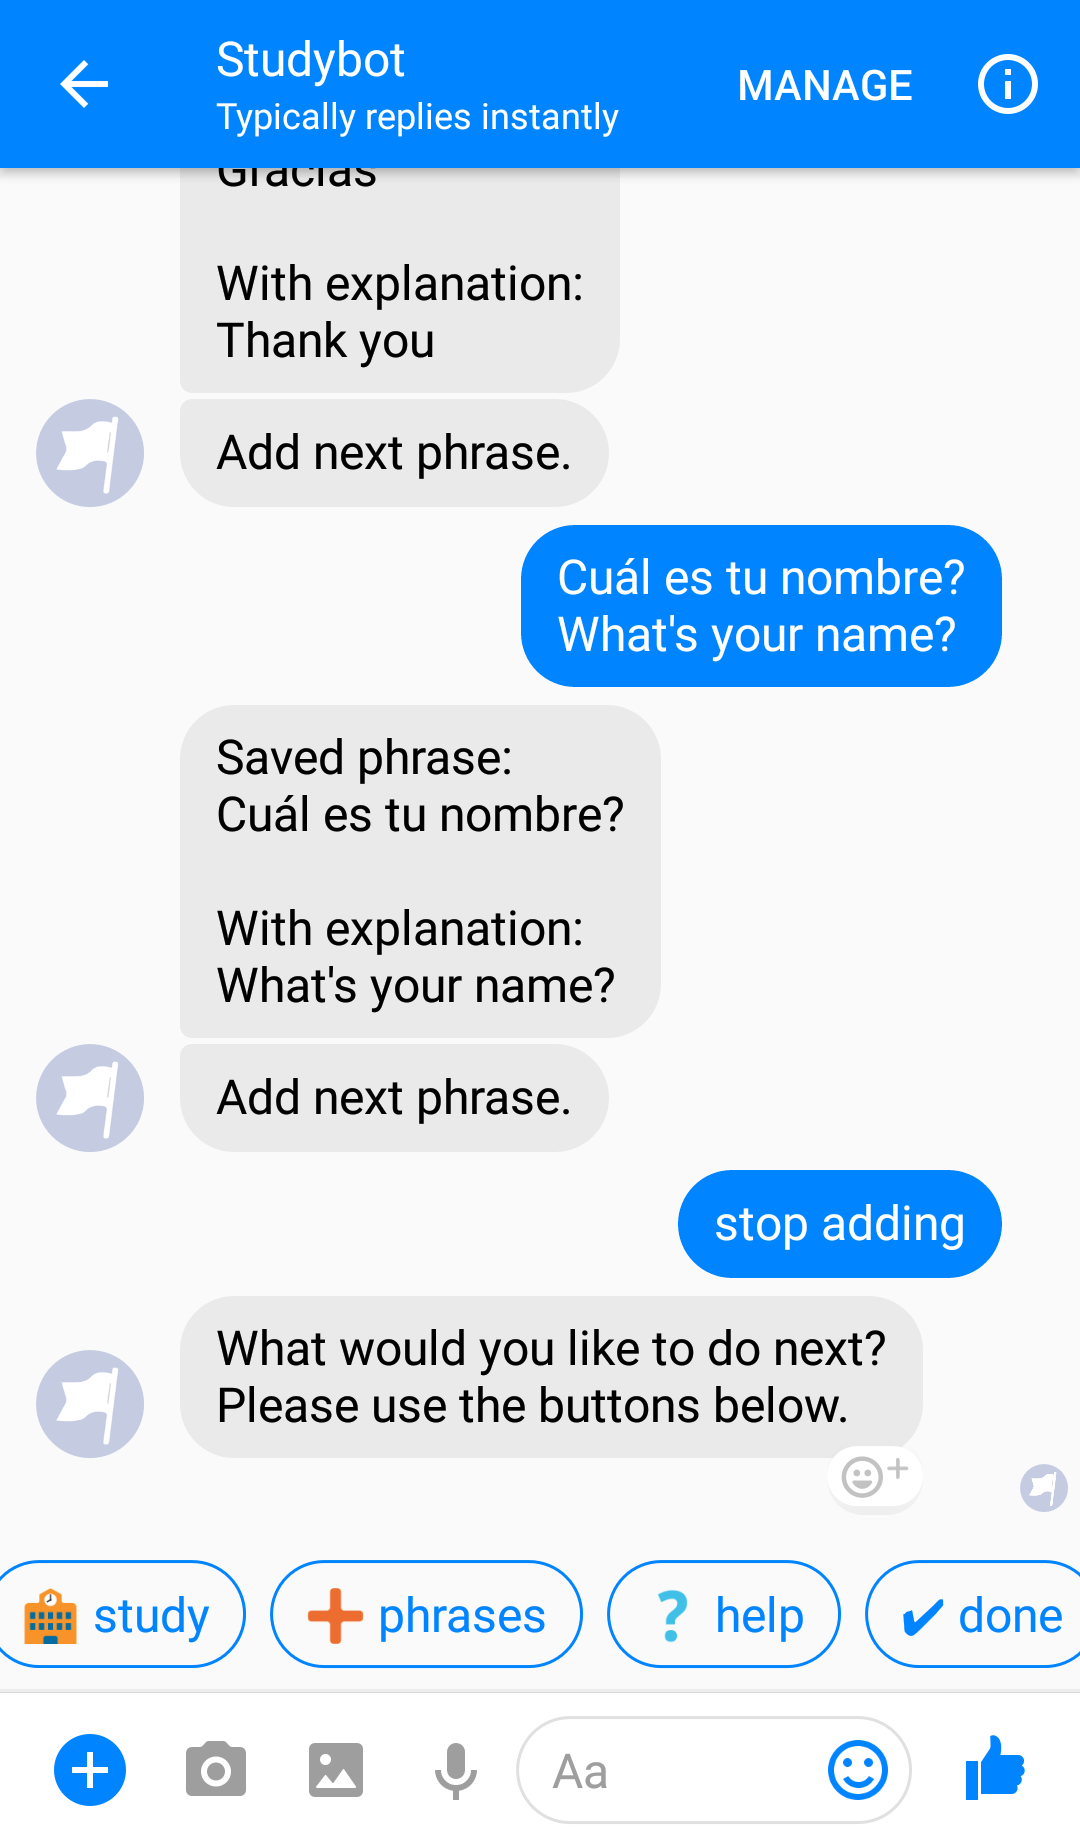
\includegraphics[width=0.28\textwidth]{images/interface/05-stop-adding.png}
	\caption{Stop adding phrases}
	\label{fig:05-stop-adding}
\end{wrapfigure}

As shown in figure \ref{fig:04-add}, three phrases have been added to Studybot
before the user decides to press the button labeled as \texbf{stop adding}.
\\
Figure \ref{fig:05-stop-adding} shows, that after stopping the adding of phrases the user is prompted with an array of four possible actions;
the actions are labeled as \textbf{study}, \textbf{+ phrases}, \textbf{help} and \textbf{done} respectively
and each button label also contains an emoji\footnote{``Emoji are pictographs (pictorial symbols) that are typically presented in a colorful form and used inline in text. They represent things such as faces, weather, vehicles and buildings, food and drink, animals and plants, or icons that represent emotions, feelings, or activities.''\cite{emoji}} used as icon for the action to make it easier identifiable for the user.
\\

The chatbot has different modes of interaction.
\\
Internally the chatbot needs to keep track of the current mode of each user to be able
to address messages in the correct context.
\\
In figure \ref{fig:05-stop-adding} the user has left the mode for adding words
and entered the \emph{menu mode} from where other modes can be accessed.
\\

\begin{figure}[h]
  \centering
  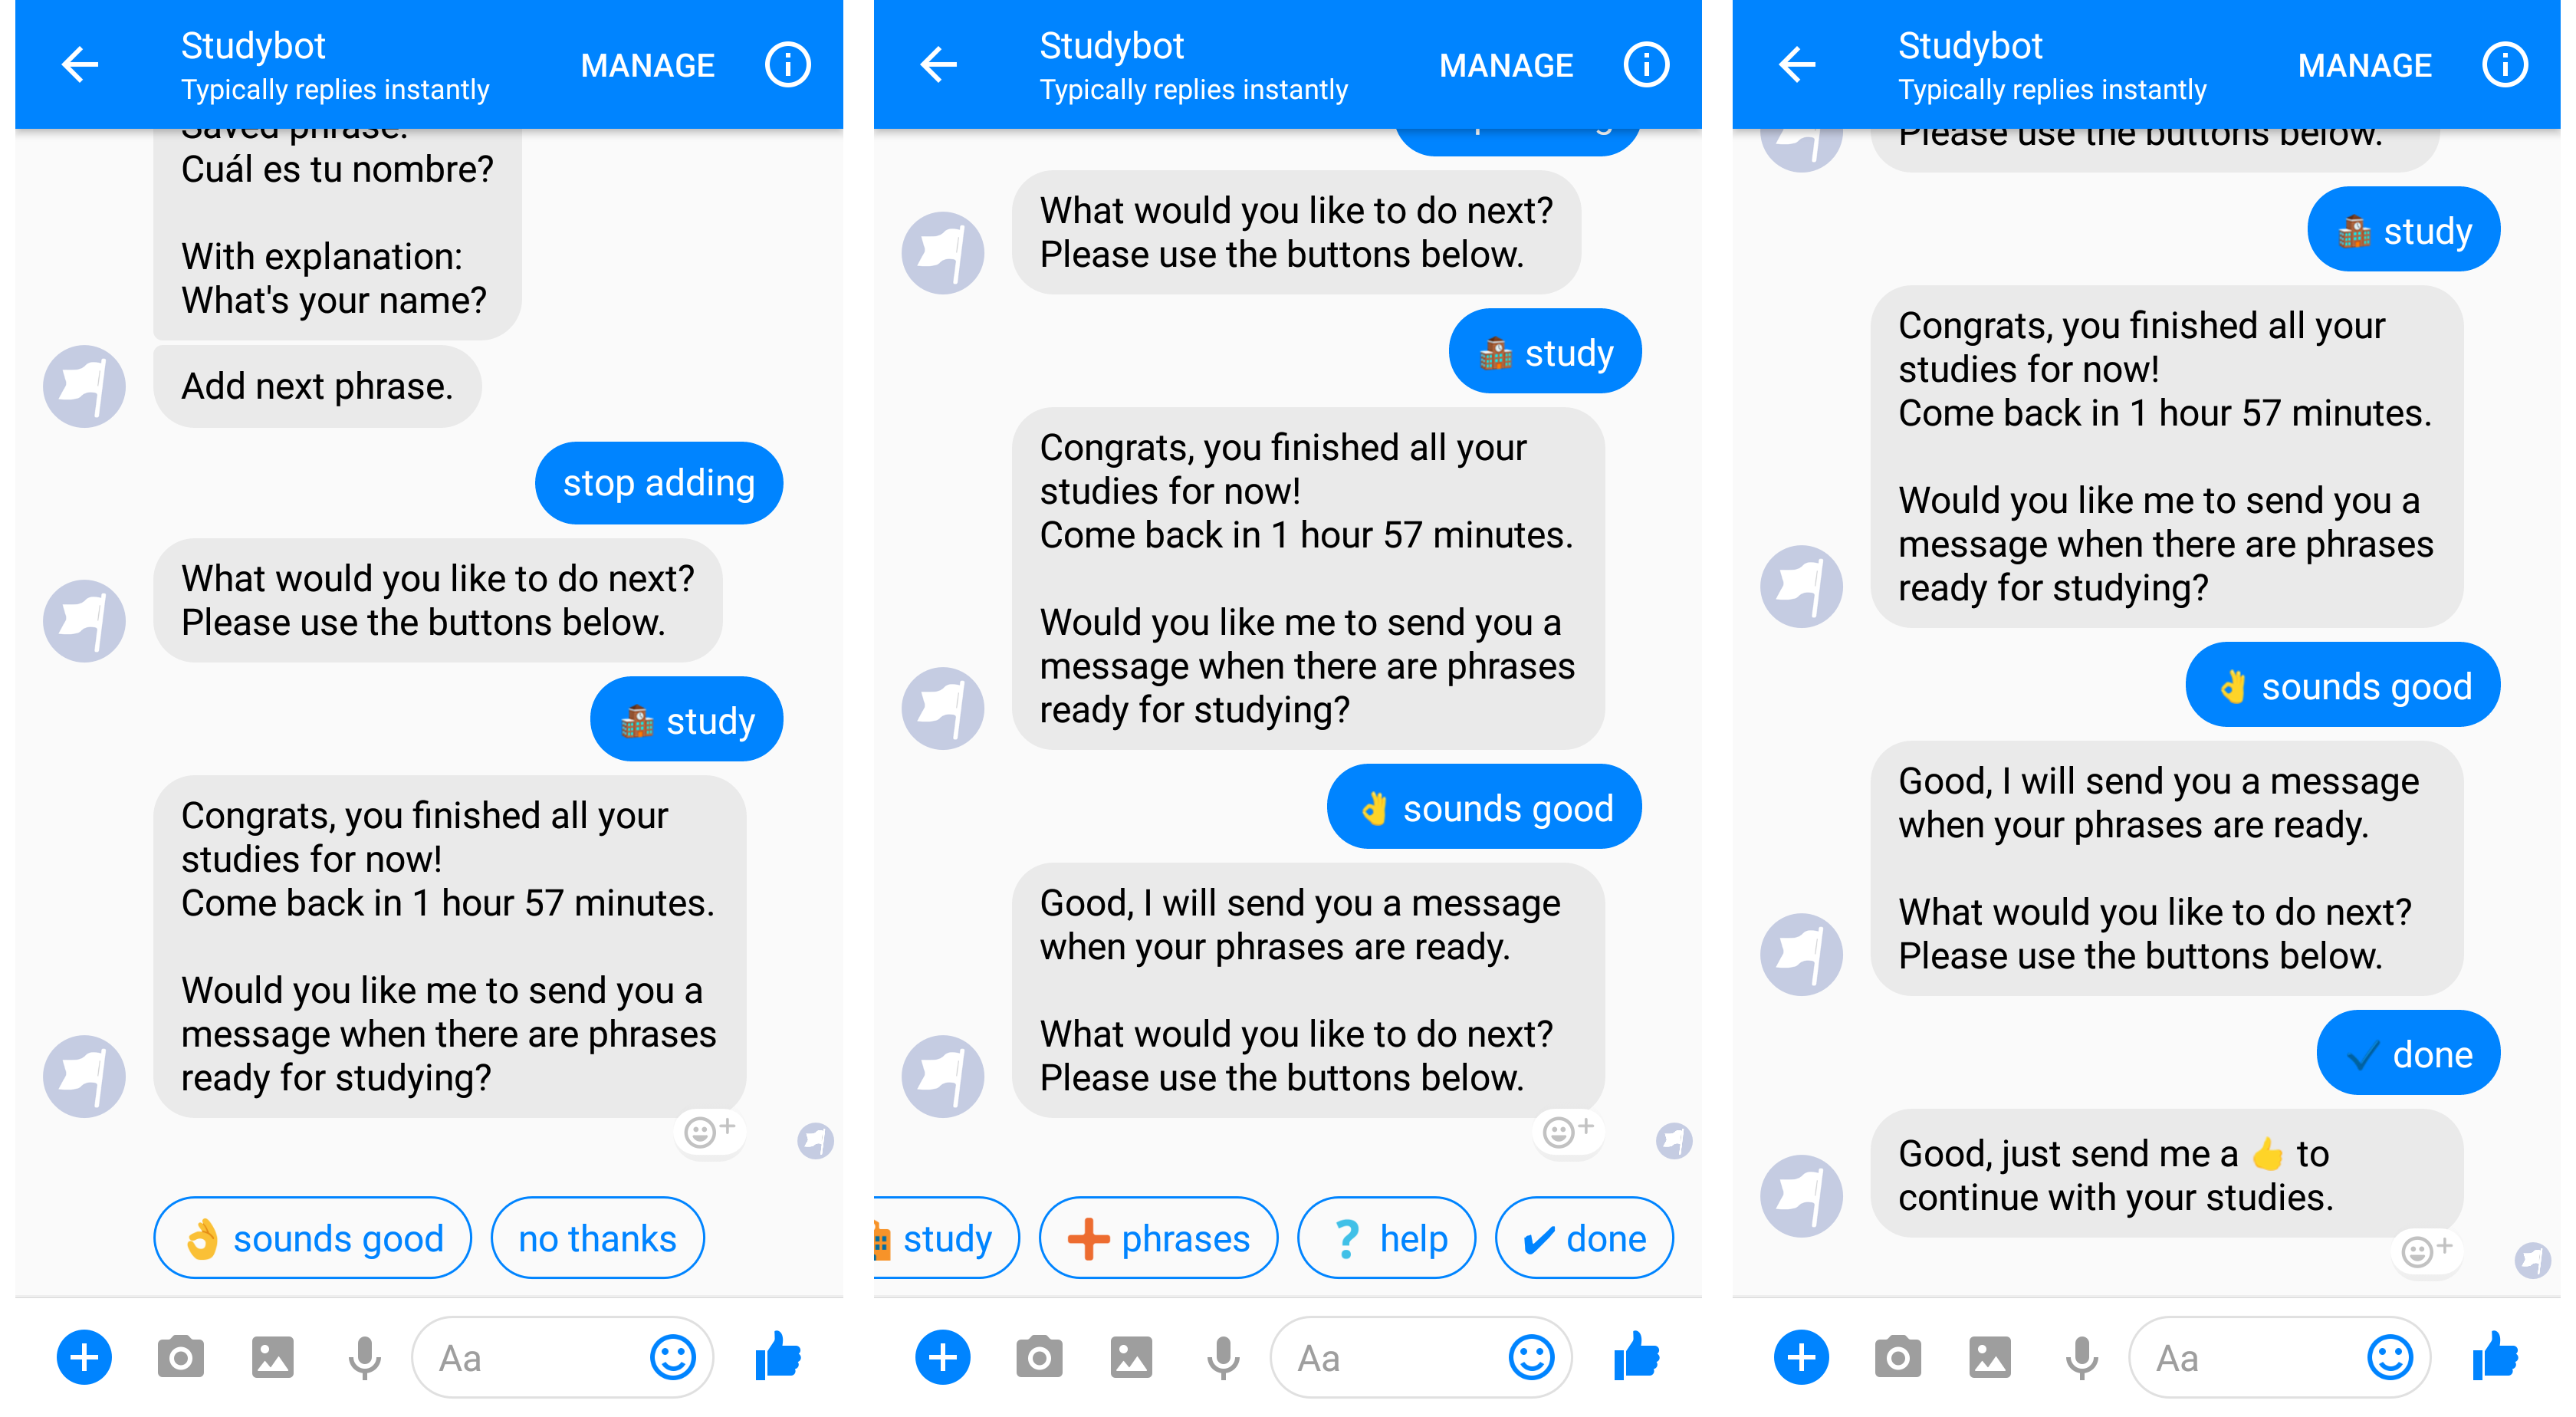
\includegraphics[width=0.9\textwidth]{images/interface/06-enable-notify.png}
	\caption{Attempt to study and activation of notifications}
	\label{fig:06-enable-notify}
\end{figure}

By clicking on the button labeled \textbf{study},
the user switches to the mode for studying of the added vocabulary.
\\
However as the image on the left of figure \ref{fig:06-enable-notify} shows,
the added phrases cannot be studied yet.
\\

Studybot uses a concept known as \emph{spaced repetition system}, or short \emph{SRS},
which is described as ``a learning technique that incorporates increasing intervals of time between subsequent review of previously learned material in order to exploit the psychological spacing effect.''\cite{srs}
\\
Based on this approach users need to wait before studying newly added vocabulary.
The more often a phrase is guessed correctly the less frequent the user will be asked to review the phrase.
\\

\begin{figure}[h]
  \centering
  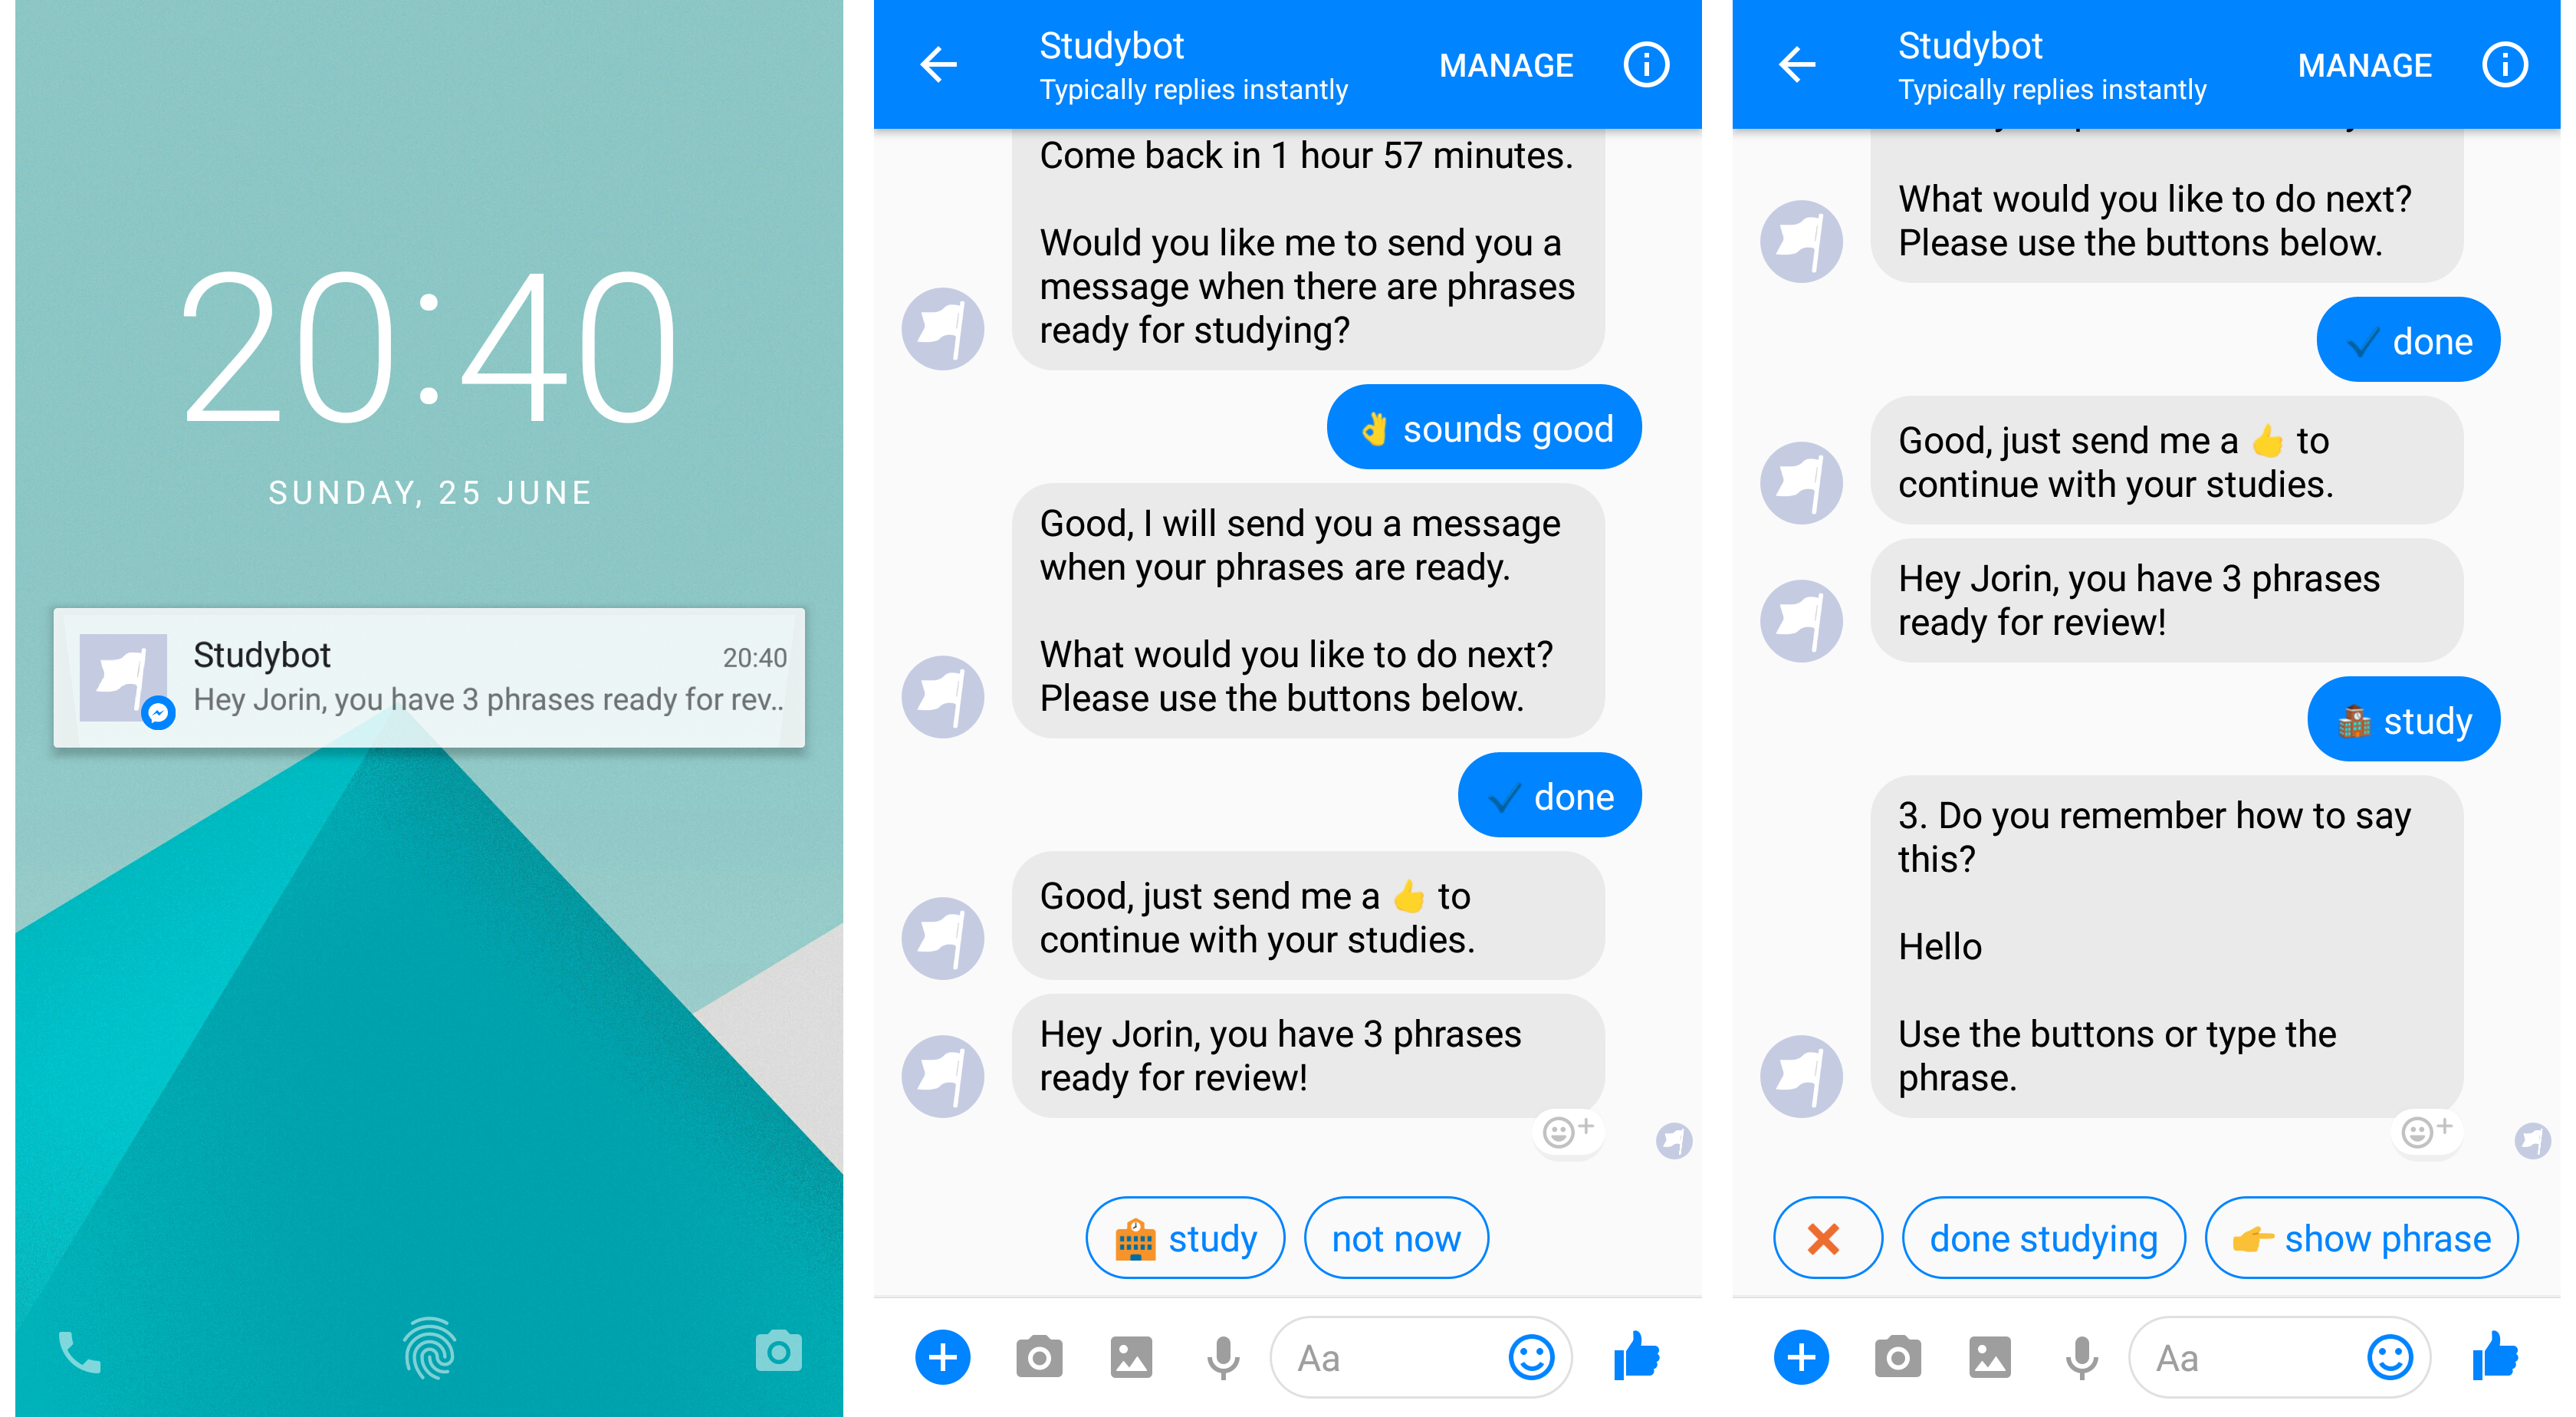
\includegraphics[width=0.9\textwidth]{images/interface/07-notify-study.png}
	\caption{Notification message and beginning of study}
	\label{fig:07-notify-study}
\end{figure}

Instead of studying the previously added phrases directly,
the user is offered to receive a notification message once phrases are ready for review.
\\

When sending notifications to users, it is important to not send more messages than necessary,
and depending on the messenger platform, there are different policies in place on how many messages are permitted.
\\
The platform policy of Facebook Messenger clearly states to
``respect all requests (either on Messenger or off) by people to block, discontinue, or otherwise opt-out of your using Messenger to communicate with them''\cite{fbpolicy},
which means there needs to be a way for users to disable the sending of notifications;
and further the platform policy clarifies that ``you may message people within 24 hours of a person's interaction with your business or Bot ..., and until the next interaction, you may send one additional message after this 24 hour period in order to follow up on your conversation.''\cite{fbpolicy}
\\

\begin{figure}[h]
  \centering
  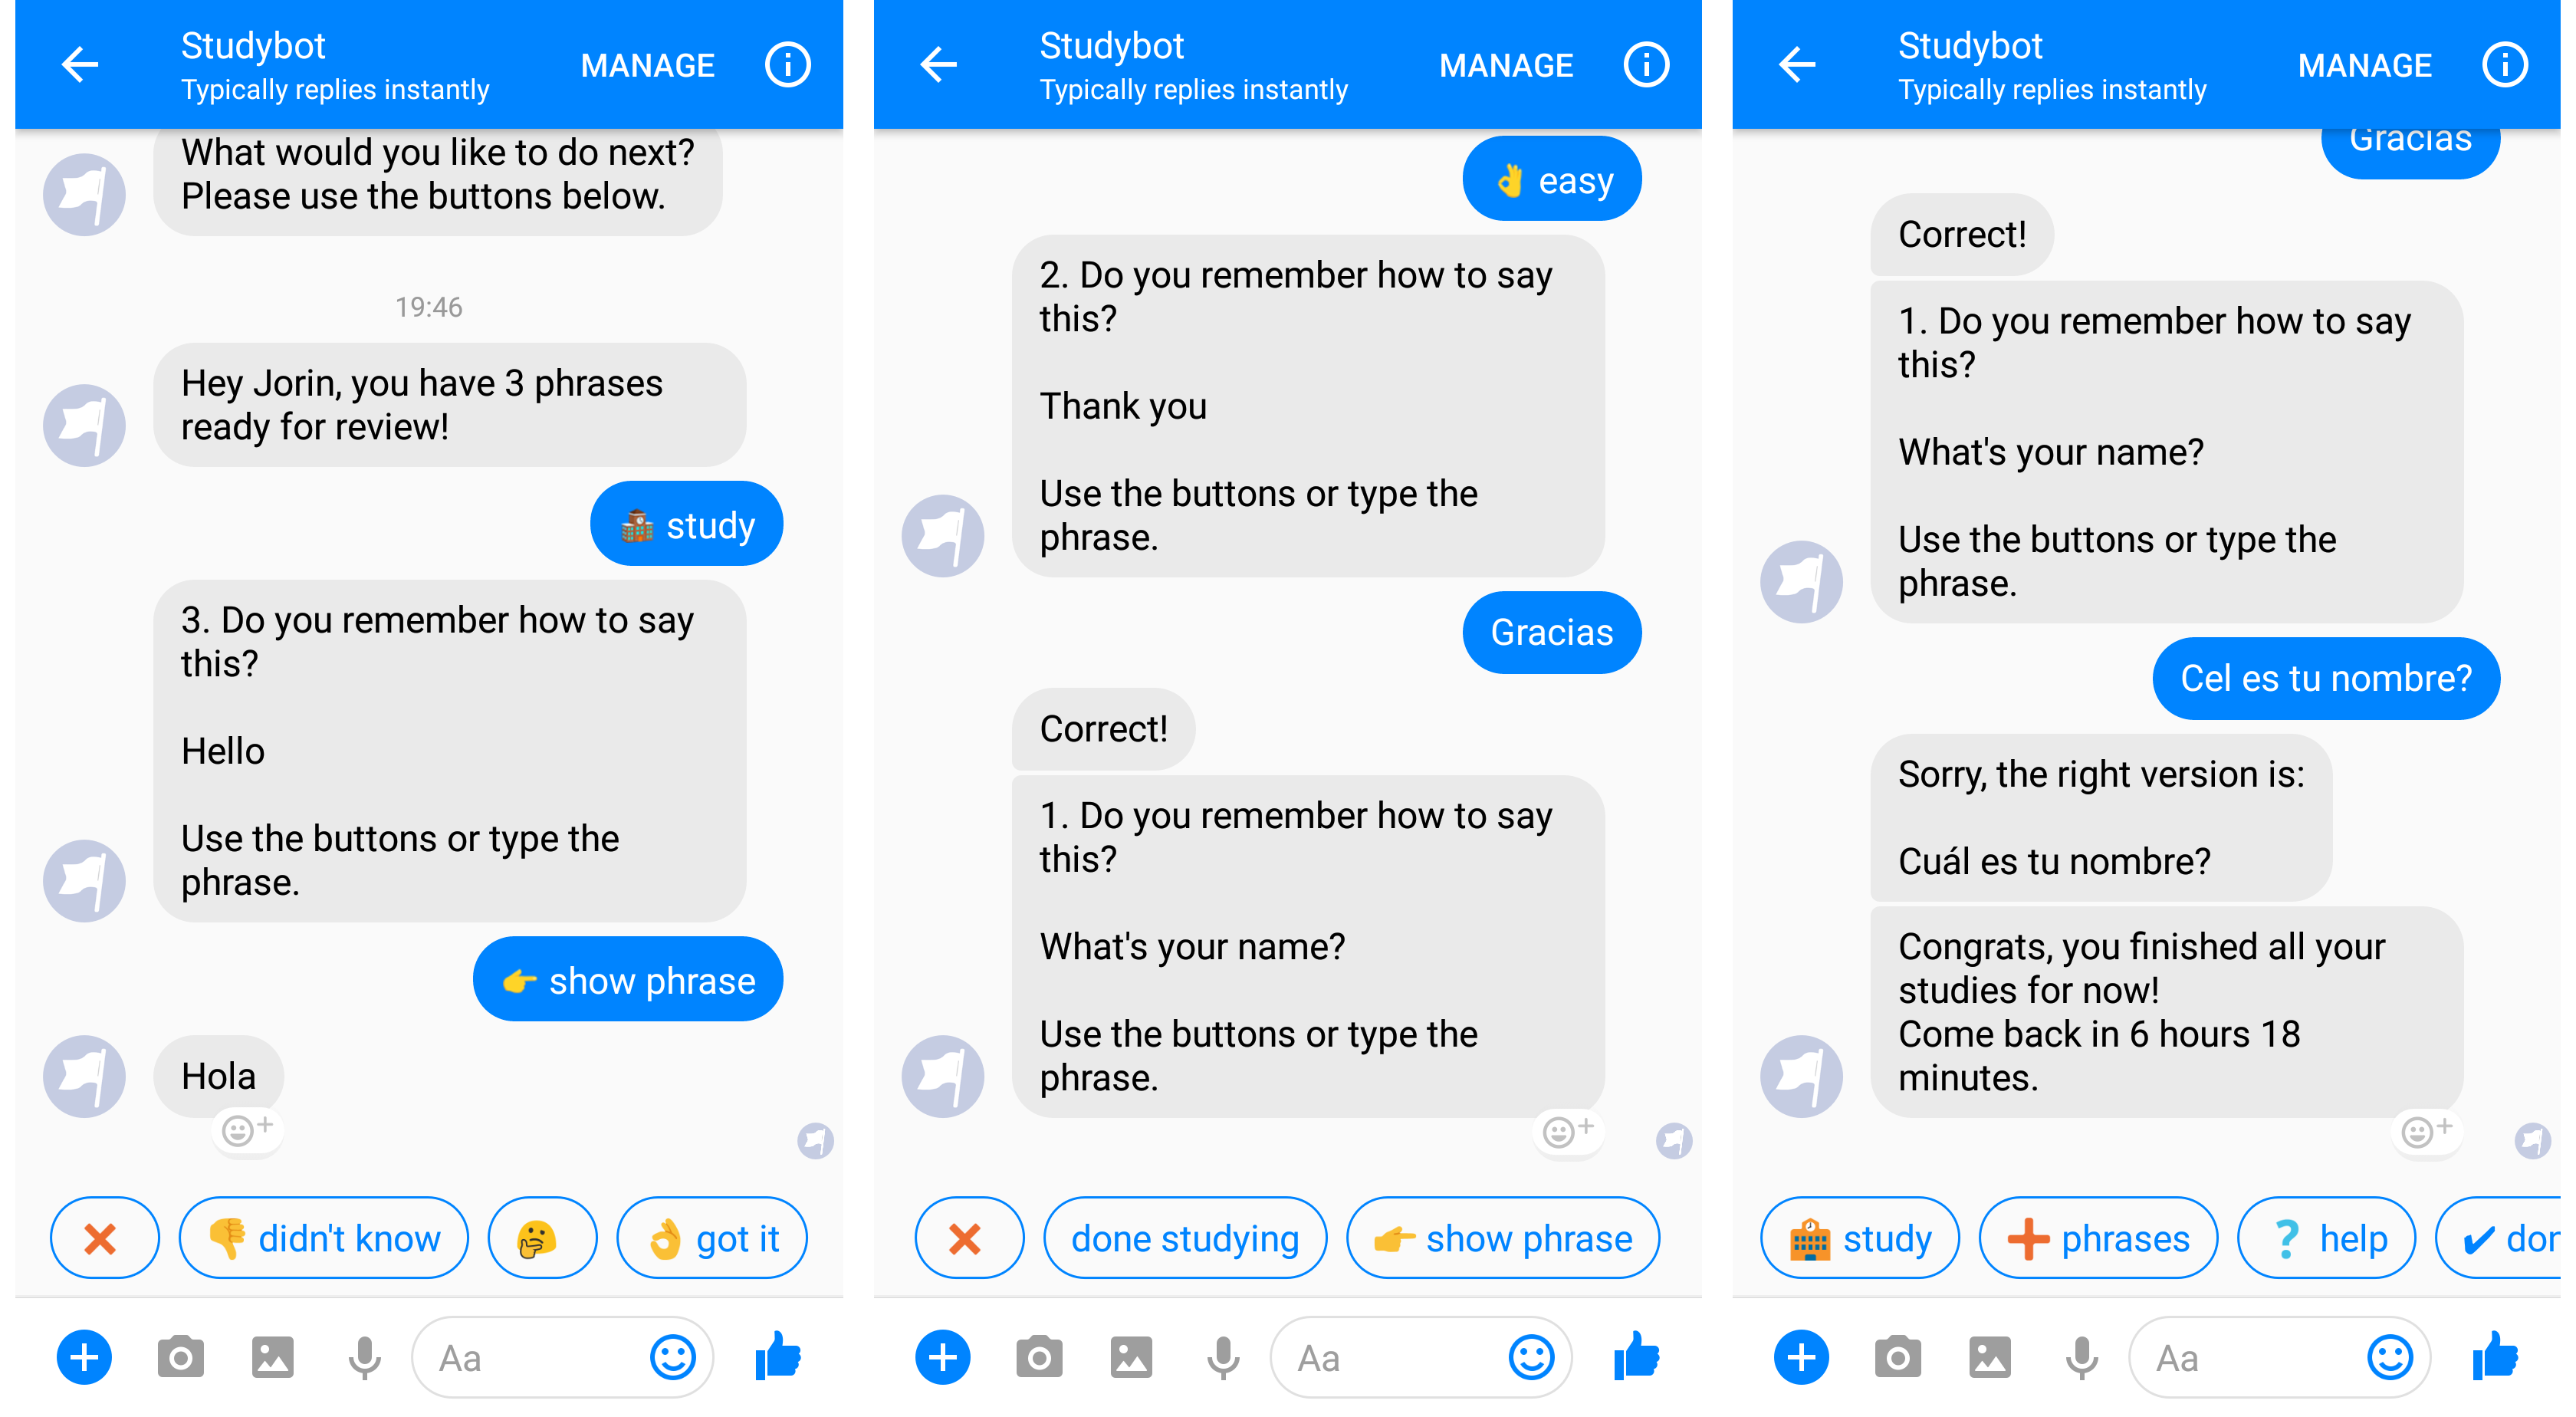
\includegraphics[width=0.9\textwidth]{images/interface/08-study-done.png}
	\caption{Study using buttons or by typing}
	\label{fig:08-study-done}
\end{figure}

In figure \ref{fig:07-notify-study} a notification on form the Messenger application on the mobile phone is how.
It is triggered when studies are ready for review.
\\
When opening the conversation with the chatbot,
the user is now prompted to study.
\\
As defined as a requirement in \ref{funcreq} on page \pageref{funcreq},
while studying one is free to choose to answer either by using the buttons at the bottom of the screen
or by directly typing the correct phrase.
\\

The \textbf{x} button available on the right image of figure \ref{fig:07-notify-study},
allows users to delete a phrase.
\\
Since there is no possibility in Facebook Messenger to display a long list of interactive elements to the user,
creating separate functionality for editing and deleting phrases is difficult to achieve,
and while studying is at this point the only possibility to refer to a phrase.
\\

The figures \ref{fig:07-notify-study} and \ref{fig:08-study-done} show a subtle decision to display the buttons users are most likely to interact with,
on the right side;
in other places it is more intuitive to show the most important information on the left,
since English language is written from left to right and we scan text accordingly;
however for certain interactions, like studying in this case, need to be performed so frequently,
a user will remember the location of the buttons quickly and doesn't need to scan process the information every single time.
\\
In this case it is helpful to have the most used action on the right side, since the majority of humans is right-handed,
therefore can reach the button with the thumb with less effort when using a mobile phone single-handed.
\\


With this the primary interactions for the example chatbot are covered.
\\
Many of the implemented interactions can be transfered and reused when creating other kinds of chatbot;
addressing the user by name,
sending text in small chunks with a time of delay in between,
prompting the user for specific input with every message,
keeping track of the user's context,
asking for permission before sending notifications and
consciously ordering buttons,
these patterns can be applied to in many different scenarios.

% TODO
% Information about secondary interactions can be found on \pageref{fig:secondary} in the appendix.


\section{Server Architecture}

The following is an overview about how the example chatbot has been created.
\\
Instead of covering all details, the focus here is to communicate the underlying concepts,
which are not unique to this specific chatbot and thereby enable others to apply similar patterns in their own development.
\\

\begin{figure}[h]
  \centering
  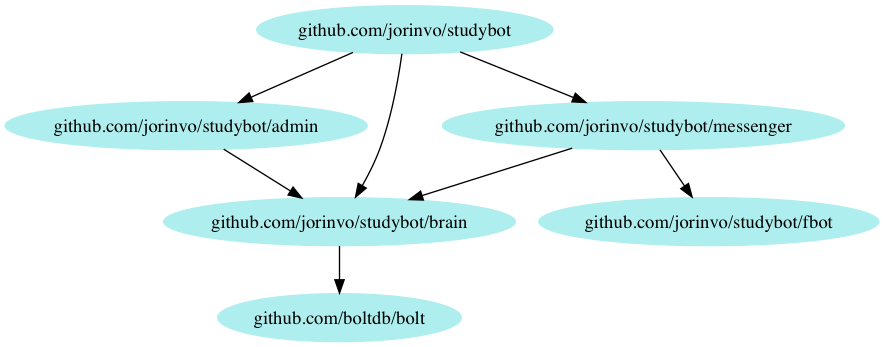
\includegraphics[width=0.8\textwidth]{images/internal-deps.png}
  \caption{Package dependency graph\footnotemark}
	\label{fig:internal-deps}
\end{figure}
\footnotetext{The graph has been created with \emph{godepgraph}\cite{godepgraph}}

There are numerous resources available today that demonstrate the development of chatbots.
However a majority of the existing material relies on specific services, frameworks or libraries for the implementation.
\\
The implementation of the example chatbot demonstrates all basics necessary for the creation of a chatbot
without relying on external tooling;
the code-base has no external dependencies, with the exception of a package for the database.
\\

The Graph in figure \ref{fig:internal-deps} shows the overall architecture of the chatbot.
\\
The \textbf{main} package handles only configuration, setup and tear-down.
It instantiates the data \emph{store} from package \textbf{brain}
and starts web servers listening on two separate ports for the packages \textbf{messenger} and \textbf{admin}.
\\

The \emph{store} has a connection to the database and it is responsible for all domain-specific business logic of \emph{Studybot}.
Both servers use the \emph{store} to fulfill their HTTP requests and they therefore depend on package \textbf{brain}.
\\
Package \textbf{admin} only provides functionality for internal use by the administrators of the chatbot;
one of its main responsibilities is to handle communication with Slack
for the in \ref{slackhook} on page \pageref{slackhook} mentioned feature.
\\

Package \textbf{messenger} is responsible for processing all events received from the Facebook Messenger platform.
\\

It relies on another package named \textbf{fbot},
which is a simple abstraction over the for this chatbot needed functionality of the Facebook Messenger platform.
Communication in this package happens via JSON over HTTP and since this is a custom package
specifically designed to be used in this chatbot, it only needs to support data types and parameters that are actually interesting to this product.
\\

\begin{figure}[h]
  \centering
  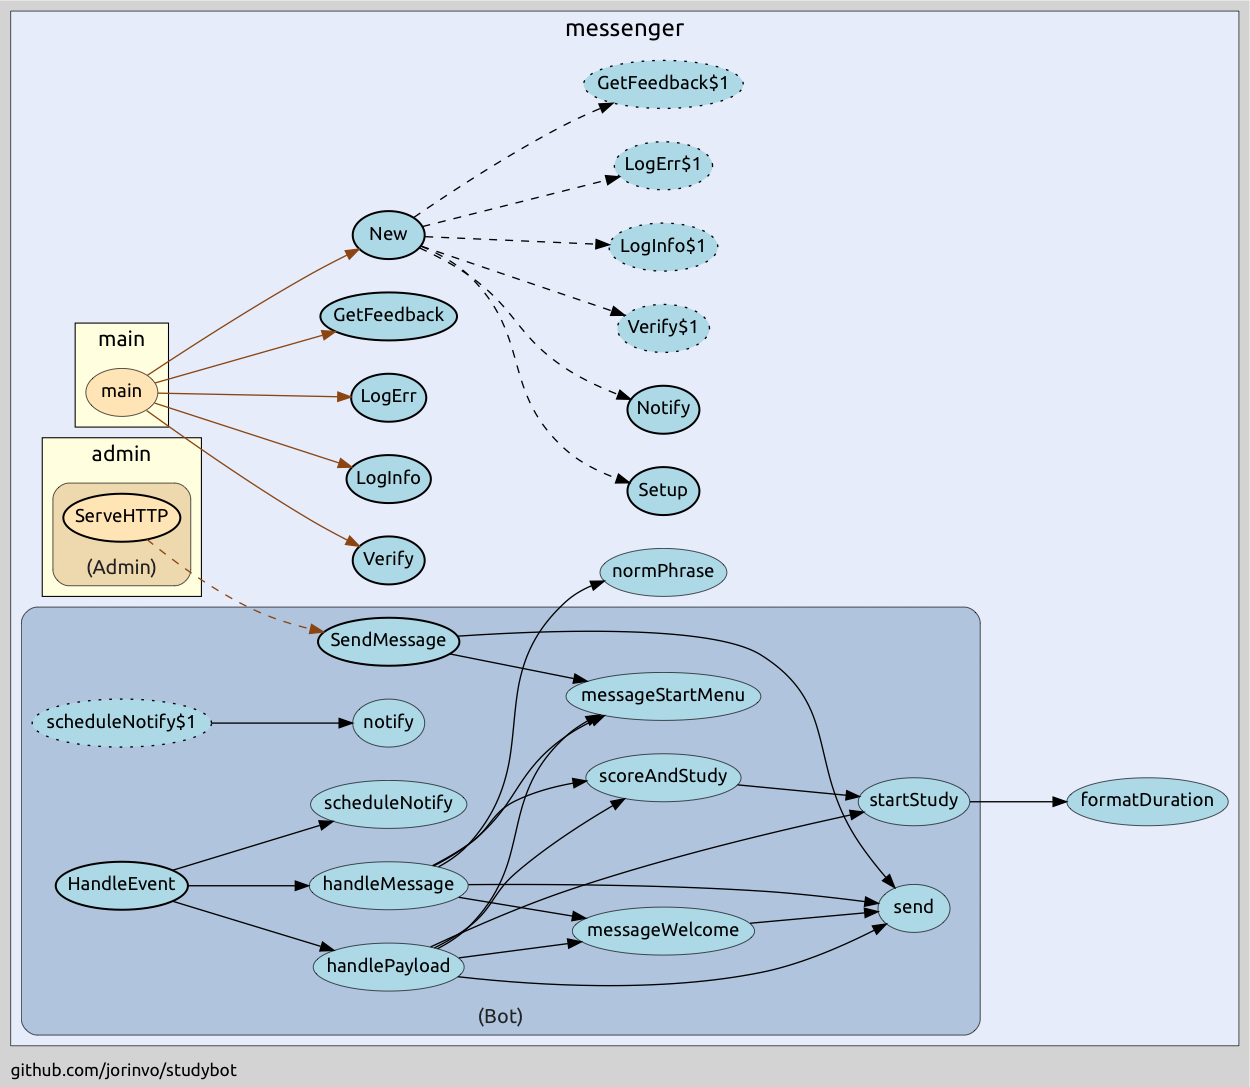
\includegraphics[width=0.8\textwidth]{images/call-graph-messenger.png}
	\caption{Call Graph of the messenger package\footnotemark}
	\label{fig:call-graph-messenger}
\end{figure}
\footnotetext{The visualization has been created with \emph{go-callvis}\cite{gocallvis}}


Most of the code-base and its architecture are structure the same way most other servers are organized,
the logic that is more specific to the development of a chatbot is mainly contained in the package \textbf{messenger}.
\\
Figure \ref{fig:call-graph-messenger} illustrates the behavior of this package,
but it should be noted that for brevity calls to the packages \textbf{brain} and \textbf{fbot} are not included in the graphic.
\\
The upper half of the graphic in \ref{fig:call-graph-messenger} shows function calls,
which are invoked from package \textbf{main} for initializing an instance of the type \emph{Bot}.
\\

The type \emph{Bot} provides functionality to handle events coming from the Facebook Messenger platform
and sending properly generated responses back to users.
\\
The function \emph{HandleEvent}, which can be seen in figure \ref{fig:call-graph-messenger},
is called by package \textbf{fbot} with every event the webhook receives,
and this is the main entry-point into the custom chatbot logic.
Depending on the type of the event,
\emph{HandleEvent} tracks whenever a user read a message,
or sends a message back to the user,
whereby it has to be differentiate between handling raw text messages
or handling the use of a predefined button and its action payload.
\\

In addition to directly responding to users,
\emph{HandleEvent} is also the source for scheduling the sending of notifications.
With every action of a user, the next time they receive a notification message needs to be rescheduled,
which happens in the call to the function \emph{scheduleNotify}.
The function in \ref{fig:call-graph-messenger} labeled as \emph{scheduleNotify\$1} is an anonymous callback function,
one for each user, that is called by the scheduled timer to send a message to the user.
\\

Further, it is visible in \ref{fig:call-graph-messenger},
that package \textbf{admin} can call a functioned named \emph{SendMessage} which belongs to the \emph{Bot} type.
This is used to send replies, that administrators created inside Slack, back to users,
since package \textbf{messenger} is the only package responsible for communicating with the Facebook Messenger platform.
\\

Limiting logic specific to the chosen platform, in this case Facebook Messenger,
makes it easier to adopt the chatbot to new platforms in the future.

% TODO
% Call graphs for the other packages can be found on \pageref{} in the appendix,
% and to further understand the generated documentation for all packages on \pageref{} can be consulted.

% \input{content/21-obstacles-and-limitations.tex}
% \input{content/22-conclusions.tex}
% \input{content/23-outlook-and-possibilities.tex}


\printbibliography[heading=bibintoc]


\chapter*{Erklärung}

Hiermit versichere ich, dass ich die vorliegende Arbeit selbstständig verfasst und keine anderen als die angegebenen Quellen und Hilfsmittel benutzt habe, dass alle Stellen der Arbeit, die wörtlich oder sinngemäß aus anderen Quellen übernommen wurden, als solche kenntlich gemacht und dass die Arbeit in gleicher oder ähnlicher Form noch keiner Prüfungsbehörde vorgelegt wurde.

\vspace{3cm}
Ort, Datum \hspace{5cm} Unterschrift\\

\end{document}
